% --- Document Class ---
\documentclass[12pt]{report} % Sử dụng class 'report' với cỡ chữ 12pt

% --- Encoding and Font ---
\usepackage[utf8]{inputenc} % Mã hóa ký tự đầu vào (hỗ trợ tiếng Việt)
\usepackage[T1]{fontenc}    % Mã hóa font chữ (quan trọng cho copy-paste và hiển thị)
\usepackage{mathptmx} % Sử dụng họ phông chữ Times New Roman (text và math)
\usepackage{seqsplit}
\usepackage{enumitem}

% --- Layout and Spacing ---
\usepackage[left=3cm, right=2.8cm, top=2.54cm, bottom=2.54cm]{geometry} % Thiết lập lề trang tùy chỉnh
\usepackage{setspace}     % Gói để điều chỉnh khoảng cách dòng
\usepackage{url}
\doublespacing            % Áp dụng giãn dòng đôi cho toàn bộ tài liệu
\usepackage{titlesec}
\setlength{\parindent}{0pt} % Bỏ thụt đầu dòng cho tất cả các đoạn văn

% --- Headers and Footers ---
\usepackage{fancyhdr}     % Gói để tùy chỉnh header và footer
\pagestyle{fancy}        % Áp dụng kiểu 'fancy' cho header/footer
\fancyhf{}               % Xóa tất cả các trường header/footer hiện tại
\fancyhead[R]{\thepage}  % Đặt số trang ở bên phải của header

% --- Graphics and Tables ---
\usepackage{graphicx}     % Gói để chèn hình ảnh (\includegraphics)
\usepackage{booktabs}     % Gói để tạo đường kẻ bảng đẹp hơn (\toprule, \midrule, \bottomrule)
\usepackage{array}        % Gói hỗ trợ định dạng cột nâng cao cho bảng (ví dụ: >{\centering})
\usepackage{float}
\usepackage{caption}
% --- Các gói khác (Thêm nếu cần) ---
% Ví dụ:
 \usepackage[vietnamese,english]{babel} % Nếu cần hỗ trợ đa ngôn ngữ hoặc các quy tắc đặc thù ngôn ngữ
% \usepackage{amsmath}       % Nếu cần các công thức toán học phức tạp
% \usepackage{hyperref}      % Để tạo liên kết có thể click (thường nên đặt cuối cùng)

% --- Thiết lập Bibliography (Thêm phương pháp bạn chọn vào đây) ---
% Ví dụ dùng BibTeX với babel:
\usepackage[english]{babel} % Đảm bảo babel được load
\usepackage{comment}
\addto\captionsenglish{\renewcommand{\bibname}{References}}
%
% Ví dụ dùng BibLaTeX:
% \usepackage[backend=biber, style=numeric]{biblatex}
% \addbibresource{references.bib} % Tên file .bib của bạn
% \DefineBibliographyStrings{english}{bibliography = {References}, references = {References}}

% --- CÁC GÓI CẦN THIẾT ---
%\usepackage[utf8]{inputenc} % Hỗ trợ gõ Unicode
\usepackage[T5]{fontenc}    % Hỗ trợ hiển thị tiếng Việt cho pdfLaTeX
%\usepackage[hidelinks]{hyperref}       % Hỗ trợ lệnh \url{} và tạo link bấm được

% --- Định dạng tiêu đề ---
%\usepackage{titlesec}

\usepackage{tikz}
\usetikzlibrary{arrows.meta, positioning}

\usepackage{amsmath}

\usepackage{pmboxdraw}

\usepackage{multirow}

% Định nghĩa các lệnh để dễ thay đổi thông tin
\newcommand{\thesistitle}{	
\textbf{A Comparative Study of BERT, LSTM, and Hybrid BERT-LSTM Models for Vietnamese Sentiment Analysis}}
\newcommand{\authorname}{Dao Van Phu}
\newcommand{\supervisor}{Dr. Bui Cao Vu}
\newcommand{\yearofconvocation}{2026}
\titleformat{\chapter}[display]
  {\normalfont\huge\bfseries\centering}
  {\chaptertitlename\ \thechapter}
  {20pt}
  {\Huge}
\titleformat{name=\chapter,numberless}[display]
  {\normalfont\huge\bfseries\centering}
  {}
  {0pt}
  {\Huge}
\begin{document}

% Trang bìa
\begin{titlepage}
    \thispagestyle{empty}
    \begin{center}
        {\large MINISTRY OF EDUCATION AND TRAINING}\\
        {\large FPT UNIVERSITY}\\
        \vspace{2cm}
        {\LARGE \thesistitle}\\
        \vspace{1cm}
        by\\
        {\large \authorname}\\

        \vspace{1cm}
        Supervisor:\\
        \supervisor\\

        \vspace{2cm}
        (C) Copyright by \authorname\ \yearofconvocation\\
    \end{center}
\end{titlepage}

% Trang tóm tắt (Abstract)
\cleardoublepage
\pagenumbering{roman}
\begin{center}
    {\large \thesistitle}\\
    {\large \authorname}\\
    Degree Master of Software Engineering\\
    FPT University\\
    \yearofconvocation\\
    \vspace{1cm}
    \textbf{Abstract}\\
\end{center}


% Lời cảm ơn (Acknowledgments)
\chapter*{Acknowledgments}
I express gratitude to my supervisors, \supervisor, for their guidance. I also thank FPT University for providing resources and my peers for their support in tackling Vietnamese NLP challenges.

% Mục lục (Table of Contents)
\tableofcontents

% Danh sách bảng (List of Tables)
\listoftables

% Danh sách hình (List of Figures)
\listoffigures

% Phần chính của luận văn
\cleardoublepage
\pagenumbering{arabic}

\chapter{Introduction}

\section{Background}

Sentiment Analysis (SA), also known as opinion mining, has become a pivotal task in Natural Language Processing (NLP), enabling organizations to automatically gauge public opinion from vast amounts of textual data. While sentiment analysis for English has reached a certain level of maturity, \textbf{Vietnamese Sentiment Analysis (VSA)} remains a challenging research frontier due to the language's unique linguistic characteristics.

\begin{itemize}
    \item \textbf{Linguistic Challenges:}
          \begin{itemize}
              \item \textbf{Word Segmentation:} Unlike English, Vietnamese is a tonal language in which meaning relies heavily on diacritics. Furthermore, it is an analytic language where word boundaries are not explicitly defined by whitespace. For example, \foreignlanguage{vietnamese}{``đất nước''} is considered
                    a single word meaning ``country'', although it is composed of two tokens, \foreignlanguage{vietnamese}{``đất''} and \foreignlanguage{vietnamese}{``nước''}.

              \item \textbf{Polysemy and Context:} The language possesses a flexible grammatical structure that relies heavily on context and diacritics (tones).

              \item \textbf{Internet Slang and "Teencode":} The prevalence of slang, abbreviations, and emoticons in informal Vietnamese communication reduces the accuracy of traditional sentiment dictionaries.
          \end{itemize}

    \item \textbf{Technological Evolution: From Traditional to Modern Approaches}

          The history of Sentiment Analysis research has witnessed a significant technological shift, particularly in the context of Vietnamese natural language processing, which presents unique challenges such as complex semantic structures, tonal diversity, and a relative scarcity of annotated linguistic resources compared to English \cite{nguyen2018vlsp, nguyen2018variants}:

          \begin{itemize}
              \item \textbf{Early Stage:} Lexicon-based methods and traditional machine learning algorithms such as \textbf{SVM} and \textbf{Naive Bayes} were widely adopted in early Vietnamese sentiment analysis research \cite{nguyen2018vlsp}. However, these approaches frequently struggled to capture deep semantics --- particularly negation structures, sarcasm, and idiomatic expressions characteristic of Vietnamese --- while relying heavily on manual feature engineering.

              \item \textbf{Deep Learning Era:} The advent of recurrent neural networks, and specifically the \textbf{BiLSTM} (Bidirectional Long Short-Term Memory) architecture, significantly improved sequence processing capabilities by retaining long-term dependencies in both the left (preceding) and right (following) contextual directions. This bidirectional modeling is especially critical for Vietnamese, where word meaning is tightly conditioned on surrounding context \cite{nguyen2018variants}.

              \item \textbf{Transformer Era:} More recently, the emergence of \textbf{PhoBERT} \cite{nguyen2020phobert} --- the first large-scale pre-trained language model specifically designed for Vietnamese, built upon the BERT (Bidirectional Encoder Representations from Transformers) architecture --- has marked a breakthrough in Vietnamese NLP. Pre-trained on large-scale Vietnamese corpora, PhoBERT enables deep bidirectional contextual understanding and has achieved State-of-the-Art (SOTA) performance across numerous Vietnamese NLP tasks, including sentiment analysis, named entity recognition (NER), and text classification.

              \item \textbf{Hybrid Approach:} To leverage the complementary strengths of both architectures, recent studies have proposed the \textbf{Hybrid PhoBERT-BiLSTM} model, which integrates PhoBERT's deep semantic representation capability with the sequential bidirectional learning mechanism of BiLSTM. This hybrid architecture has demonstrated promising improvements in sentiment analysis performance on domain-specific Vietnamese datasets, including social media content and product reviews \cite{dang2023hybrid}.
          \end{itemize}

    \item \textbf{Practical Application Context in Vietnam:}
          Besides linguistic complexity and technological shifts, the research is driven by an urgent demand from the Vietnamese industry. The rapid digitization of the economy has led to an explosion of user-generated content that requires automated analysis:
          \begin{itemize}
              \item \textit{E-commerce Boom:} According to the \textit{Vietnam E-Business Index (EBI) 2024} by VECOM, Vietnam's e-commerce sector has sustained a growth rate of over 25\%, reaching a market scale of \$25 billion \cite{vecom_2024}. This volume renders manual feedback processing obsolete.
              \item \textit{Banking \& Fintech:} A 2024 report by Reputa (Viettel) indicates that leading banks such as Vietcombank and MBBank are aggressively deploying social listening to monitor brand health. The report highlights a significant surge in digital banking discussions, necessitating real-time sentiment detection to handle customer complaints \cite{reputa_2024}.
              \item \textit{Education Quality Assurance:} In the educational sector (the domain of the UIT-VSFC dataset), institutions are increasingly adopting data-driven approaches to analyze student feedback for accreditation and quality improvement \cite{younet_2023}.
          \end{itemize}
          This practical context validates the necessity of developing a high-performance model like the Hybrid PhoBERT-BiLSTM to solve real-world problems in Vietnam.
\end{itemize}

\section{Rationale}

While PhoBERT has demonstrated superior representational power, it requires substantial computational resources and significant training time. Conversely, BiLSTM is more lightweight and specialized for sequential data but is less effective at representing complex contexts. A potential direction is to combine both: utilizing PhoBERT to generate high-quality contextual embeddings and BiLSTM to capture local sequential features (Hybrid PhoBERT-BiLSTM).

However, the critical question remains: \textit{Does this combination truly yield superior efficacy compared to using PhoBERT or BiLSTM individually, specifically within the context of the Vietnamese language?} Currently, direct and detailed comparative studies of these three architectures on Vietnamese datasets are limited. Therefore, the topic \textbf{``A Comparative Study of BERT, LSTM, and Hybrid BERT-LSTM Models for Vietnamese Sentiment Analysis''} was chosen to provide a comprehensive, empirical, and scientifically grounded perspective, assisting in identifying the most suitable model architecture for Vietnamese sentiment analysis tasks.

\section{Motivation}

The motivation for this study stems from three critical observations in the current landscape of Vietnamese Natural Language Processing (NLP):

\begin{itemize}
    \item \textbf{The Gap Between Research and Practical Deployment:} While pre-trained Transformer-based language models such as PhoBERT have achieved state-of-the-art results, they are computationally expensive and memory-intensive. For many Small and Medium-sized Enterprises (SMEs) in Vietnam, deploying such heavy models for real-time sentiment analysis is often cost-prohibitive. There is a pressing need to determine whether lighter architectures (like BiLSTM) or hybrid approaches can offer a ``good enough'' performance with significantly lower resource consumption.

    \item \textbf{Ambiguity in Hybrid Model Efficacy:} In recent literature, combining Convolutional Neural Networks (CNN) or LSTM-based layers with BERT-family embeddings is a popular trend. However, theoretical justification for these hybrid architectures often remains vague. It is unclear whether the performance gain (if any) comes from the architectural combination or simply from the powerful PhoBERT embeddings. A rigorous comparative study is required to validate whether the complexity of a Hybrid PhoBERT-BiLSTM model is justified by a statistically significant improvement in accuracy for the Vietnamese language.

    \item \textbf{Linguistic Specificity:} Most comparative studies on Deep Learning vs. Transformers focus on English datasets (e.g., IMDB, SST-2). Due to the unique characteristics of Vietnamese grammar (word segmentation, tonal dependence), findings from English-based research cannot be blindly generalized to Vietnamese tasks. This study aims to fill this empirical gap by providing benchmarks specifically tailored to Vietnamese sentiment analysis.
\end{itemize}

\section{Research Problem}

This research focuses on resolving the following core issues:
\begin{enumerate}
    \item The capability of feature extraction and semantic representation of a Deep Learning model (BiLSTM) compared to a Pre-trained Language Model (PhoBERT) in the Vietnamese environment.
    \item The empirical effectiveness of the Hybrid architecture: Does stacking a BiLSTM layer after PhoBERT embeddings improve classification accuracy, or does it merely increase model complexity without significant benefits (diminishing returns)?
    \item The trade-off between prediction performance and computational resources when deploying these models.
\end{enumerate}

\section{Research Objectives}
The primary objective of this study is to conduct a rigorous comparative analysis of three distinct deep learning architectures to identify the optimal balance between performance and computational cost for VSA. Specifically, we aim to:
\begin{enumerate}
    \item \textbf{Evaluate Baseline Performance:} Assess the efficacy of a traditional sequential model (\textbf{BiLSTM}) versus a state-of-the-art pre-trained Transformer model (\textbf{PhoBERT}).
    \item \textbf{Develop a Hybrid Architecture:} Propose and implement a \textbf{Hybrid PhoBERT-BiLSTM} model that combines the contextual embedding power of PhoBERT with the sequential feature extraction of BiLSTM.
    \item \textbf{Trade-off Analysis:} Compare these models not only on accuracy/F1-score but also on training time and resource consumption.
    \item \textbf{Addressing Real-world Practical Problems:}
          The research specifically targets the critical pain points currently faced by Vietnamese enterprises (Banking, E-commerce, EdTech) identified in the background section:
          \begin{itemize}
              \item \textit{Scalability Solution:} Addressing the ``Data Deluge'' problem where manual analysis is impossible due to the exponential growth of feedback (growing 25\% annually). The model aims to automate the processing of thousands of comments in real-time.
              \item \textit{Nuance Interpretation:} Overcoming the limitations of current keyword-based tools that fail to detect sarcasm, teencode, or negation in Vietnamese (e.g., \foreignlanguage{vietnamese}{``ngân hàng làm ăn chán thật''} vs. \foreignlanguage{vietnamese}{``chán chả buồn nói''}). The study aims to provide a tool capable of understanding deep semantic context for accurate brand reputation management.
          \end{itemize}

    \item \textbf{Research Questions (RQs):}
          To guide the comparative analysis, this study formulates the following core research questions:
          \begin{itemize}
              \item \textbf{RQ1:} To what extent does the Hybrid PhoBERT-BiLSTM architecture outperform standalone models (BiLSTM and PhoBERT) in classifying Vietnamese sentiment?
              \item \textbf{RQ2:} How effective is the combination of PhoBERT's contextual embedding and BiLSTM's sequential memory in handling Vietnamese linguistic complexities (e.g., word ambiguity, negation)?
              \item \textbf{RQ3:} What is the trade-off between classification accuracy and computational latency when deploying these models in a real-world application context?
          \end{itemize}
\end{enumerate}

\section{Dataset and Scope}
To ensure the study is grounded in high-quality, standardized data, the project utilizes the following data sources:

\subsection{Training Data (UIT-VSFC)}
We train and validate our models using the \textbf{UIT-VSFC} (Vietnamese Students' Feedback Corpus).
\begin{itemize}
    \item \textbf{Size:} Approximately 16,000 sentences.
    \item \textbf{Domain:} University student feedback on lecturers, facilities, and curriculum.
    \item \textbf{Original Labels:} The corpus originally provides three sentiment classes: \textit{Positive}, \textit{Negative}, and \textit{Neutral}.
    \item \textbf{Scope of This Study:} To focus the comparative analysis on clearly polarized sentiment and avoid the ambiguity and severe class imbalance associated with the Neutral category in this corpus, this study restricts the task to \textbf{binary classification (Positive/Negative)}. Samples labeled Neutral are excluded from training and evaluation across all three models.
    \item \textbf{Rationale:} This dataset is widely recognized as a benchmark for VSA, ensuring our results are comparable to existing literature.
\end{itemize}

\subsection{Testing Data (AIVIVN-2019)}
To assess cross-domain generalization beyond the academic setting of UIT-VSFC, we additionally evaluate our trained models on \textbf{AIVIVN-2019}, a Vietnamese e-commerce review dataset.
\begin{itemize}
    \item \textbf{Size:} Approximately 16,000 labeled reviews.
    \item \textbf{Domain:} User reviews of products on e-commerce platforms.
    \item \textbf{Labels:} Two sentiment classes: \textit{Positive} and \textit{Negative}, consistent with the binary scope adopted in this study.
    \item \textbf{Source:} Originally released as part of the AIVIVN 2019 Sentiment Analysis Challenge, in which the official test-set labels were kept private by the competition organizers. For this study, a publicly available, labeled version of the test set --- shared by the community on Kaggle --- is used, allowing direct quantitative evaluation without the need for manual annotation.
    \item \textbf{Rationale:} As a review dataset from a different domain (e-commerce) and register (informal customer reviews) than UIT-VSFC (semi-formal academic feedback), AIVIVN-2019 serves as an out-of-domain test bed to evaluate whether models trained on UIT-VSFC generalize to a practically relevant application context.
\end{itemize}

\subsection{Real-world Prediction (Data Crawling)}
To further test the model's robustness in a fully ``wild'' environment, unlabeled comments are collected from a real-world social media source for prediction.
\begin{itemize}
    \item \textbf{Source:} Public comments collected from a selected YouTube video, retrieved via the official \textbf{YouTube Data API}.
    \item \textbf{Tools:} Python-based data collection using the YouTube Data API v3.
    \item \textbf{Goal:} This phase demonstrates the selected model's ability to generalize to informal, unstructured, slang-heavy text typically found in social media comments, which may differ substantially from both the clean academic feedback in UIT-VSFC and the structured product reviews in AIVIVN-2019.
\end{itemize}

\chapter{Literature Review}

\section{Related Work}

The landscape of Vietnamese Sentiment Analysis (VSA) has shifted from lexicon-based and traditional machine learning methods to advanced deep learning architectures, mirroring the broader trajectory of NLP research.

\subsection{Recurrent Neural Networks (RNNs) in Vietnamese}

Prior to the Transformer era, RNNs and Long Short-Term Memory (LSTM) networks \cite{hochreiter1997lstm} were the standard approach for handling the sequential nature of Vietnamese text.

\begin{itemize}
    \item \textbf{BiLSTM Efficiency:} Nguyen et al. \cite{nguyen2018ensemble} demonstrated that Bidirectional LSTMs (BiLSTM) and related recurrent variants significantly outperformed standard RNNs and Support Vector Machines (SVMs) on Vietnamese sentiment datasets (AIVIVN 2019 and a self-collected e-commerce dataset) by capturing context from both directions simultaneously.

    \item \textbf{Embedding Limitations:} However, these models relied on static word embeddings such as Word2Vec \cite{mikolov2013word2vec}. Such embeddings assign a fixed vector to each word, failing to capture the polysemous nature of Vietnamese --- for example, distinguishing \foreignlanguage{vietnamese}{``chín''} as ``nine'' versus ``ripe'' depending on context.
\end{itemize}

\subsection{Transformer-Based Models}

The introduction of the Transformer architecture revolutionized NLP by employing self-attention mechanisms to model context without relying on sequential recurrence.

\begin{itemize}
    \item \textbf{BERT:} Devlin et al. \cite{devlin2018bert} introduced BERT, which generates context-sensitive embeddings through deep bidirectional pretraining. While powerful, the multilingual version (mBERT) often struggled with Vietnamese word boundaries and diacritic-sensitive semantics.

    \item \textbf{PhoBERT:} To address this limitation, Nguyen and Nguyen \cite{nguyen2020phobert} released PhoBERT, a monolingual model pretrained on 20GB of Vietnamese text. Experiments on the UIT-VSFC dataset \cite{nguyen2018uitvsfc} showed that PhoBERT achieves state-of-the-art accuracy, effectively handling Vietnamese diacritics and compound words.
\end{itemize}

\subsection{Hybrid Approaches}

Recent studies have explored hybrid architectures that combine deep contextual feature extraction with the sequence modeling capability of recurrent networks such as BiLSTM \cite{dang2023hybrid}. While a standard PhoBERT classifier relies solely on the \texttt{[CLS]} token representation, hybrid models instead feed the full sequence of PhoBERT embeddings into a BiLSTM layer. This approach aims to capture long-range dependencies in complex feedback paragraphs that may be missed when relying on the \texttt{[CLS]} token alone.

\subsection{Summary of Recent Studies}

To provide a comprehensive view of the current research landscape, Table~\ref{tab:related-work} summarizes key studies in Vietnamese Sentiment Analysis over recent years. The comparison highlights the transition from traditional deep learning to Transformer-based approaches and identifies existing limitations that this study aims to address.

\begin{table}[h]
    \centering
    \caption{Comparison of Recent Related Works in Vietnamese Sentiment Analysis}
    \label{tab:related-work}
    \begin{tabular}{|p{2.3cm}|p{2.2cm}|p{2.1cm}|p{1.7cm}|p{4cm}|}
        \hline
        \textbf{Study}                                    & \textbf{Model}                         & \textbf{Dataset}                        & \textbf{Key Results}                        & \textbf{Limitations}                                                                                                         \\
        \hline
        Nguyen et al. (2018) \cite{nguyen2018nics}        & BiLSTM (vs. Naive Bayes, MaxEnt, LSTM) & UIT-VSFC                                & F1: 92.0\%                                  & Compared only against traditional ML/DL baselines; lacks contextual (pretrained) embeddings.                                 \\
        \hline
        Nguyen and Nguyen (2020) \cite{nguyen2020phobert} & PhoBERT (Base)                         & UIT-VSFC                                & F1: 92.3\%                                  & High computational cost and latency; requires heavy hardware resources for deployment.                                       \\
        \hline
        Dang et al. (2023) \cite{dang2023hybrid}          & Hybrid CNN-LSTM(-SVM)                  & USAL-UTH (Shopee) \& UIT-VSFC           & Acc: 93.94\% (USAL-UTH), 93.53\% (UIT-VSFC) & Modest gain (\textasciitilde0.6\%) over standalone DNN/SVM; does not incorporate pretrained language models (e.g., PhoBERT). \\
        \hline
        Le et al. (2022) \cite{le2022kse}                 & BiLSTM + fastText                      & UIT-ViSFD (Smartphone e-commerce, ABSA) & F1: 84.48\% (aspect), 63.06\% (sentiment)   & Sentiment-level F1 markedly lower than aspect-level; an ABSA setting, so not directly comparable to sentence-level SA.       \\
        \hline
    \end{tabular}
\end{table}

As shown in Table~\ref{tab:related-work}, while PhoBERT achieves state-of-the-art results, its computational cost remains a barrier to deployment. Conversely, traditional BiLSTM-based models are lighter but lack the semantic depth of pretrained Transformer representations. This reinforces the motivation for a hybrid architecture that leverages the complementary strengths of both paradigms.

\section{Research Gap}

Despite the substantial progress achieved in Vietnamese Sentiment Analysis (VSA) over the past decade, a critical review of the recent literature reveals four specific limitations that remain insufficiently addressed by existing work.

\subsection*{Gap 1: Lack of Direct Comparison on a Unified Pipeline}

A large proportion of prior studies concentrate on optimizing a single architectural family in isolation --- either refining traditional deep learning models such as BiLSTM and its variants, or fine-tuning a single Transformer-based model such as PhoBERT --- rather than comparing multiple architectures under identical experimental conditions. Van Thin et al.\ \cite{thin2023vietnamese} explicitly note that, prior to their work, no study had evaluated multiple pretrained language models on the same set of Vietnamese sentiment datasets, since different models are typically trained with different architectures, pretraining corpora, and preprocessing steps, which makes their reported results difficult to compare fairly. While their study addresses this gap for pretrained Transformer models specifically, it does not extend the comparison to lightweight sequential architectures such as BiLSTM, nor to hybrid Transformer--RNN architectures. Consequently, there remains a scarcity of research that conducts a rigorous, side-by-side comparison of a traditional BiLSTM, a pretrained PhoBERT, and a Hybrid PhoBERT-BiLSTM model within a single, identical preprocessing and evaluation pipeline on the standard UIT-VSFC benchmark. This absence of a controlled experimental environment makes it difficult for practitioners and researchers to attribute observed performance differences strictly to architectural choice, rather than to incidental differences in preprocessing, tokenization, or evaluation protocol across studies.

\subsection*{Gap 2: Absence of Performance Analysis by Sequence Length}

Current benchmarking practice in Vietnamese sentiment analysis typically reports only aggregate, corpus-level metrics such as overall Accuracy or macro F1-score \cite{ieee2023challenges}, without disaggregating performance by input characteristics such as sentence length. This is a notable omission, since short, impulsive comments (e.g., single-clause student feedback) and long, detailed reviews place very different demands on a model's ability to retain context: a short sentence may be classified correctly from a few salient keywords alone, whereas a long passage may require tracking dependencies across multiple clauses, including negation and contrastive conjunctions that can reverse the overall polarity. Because existing studies do not report performance stratified by sequence length, it remains unclear whether the additional architectural complexity of a Hybrid PhoBERT-BiLSTM model yields a measurable advantage specifically on longer inputs where BiLSTM's sequential memory could complement PhoBERT's contextual embeddings, or whether such complexity is unnecessary overhead when applied uniformly across both short and long inputs.

\subsection*{Gap 3: Limited Generalization Assessment}

Most existing Vietnamese sentiment analysis models are trained and evaluated strictly within a single domain, typically using a train/test split drawn from the same corpus and register. Ha et al.\ \cite{ha2016lifelong} highlight that sentiment classifiers trained on one domain (e.g., product reviews) often degrade substantially when applied to review text from a different domain, since sentiment-bearing vocabulary and expression patterns can shift considerably across domains --- a challenge that becomes more pronounced for Vietnamese, given the added variability introduced by informal internet slang and teencode in social media text. However, this line of work primarily addresses domain adaptation for lexicon-based or shallow models, and does not evaluate how a modern Hybrid PhoBERT-BiLSTM architecture generalizes when transferred, without any retraining, from a semi-formal academic domain (UIT-VSFC) to a structured but stylistically distinct e-commerce review domain (AIVIVN-2019), or to fully unstructured, informal social media text of the kind collected via the YouTube Data API in this study (see Section~1.6.3). This dual-source, cross-domain evaluation design allows the present study to assess generalization along two distinct axes: domain shift with preserved label availability (AIVIVN-2019), and domain shift combined with the absence of ground-truth labels in an uncontrolled ``wild'' setting (YouTube comments).

\subsection*{Gap 4: Neglect of Deployment Constraints (Latency \& Model Size)}

While recent research continues to pursue incremental gains in state-of-the-art (SOTA) accuracy \cite{ieee2023challenges}, computational efficiency is frequently treated as a secondary concern rather than a primary evaluation criterion. Pretrained Transformer models such as PhoBERT, while highly accurate, carry substantially larger parameter counts and higher inference latency than lightweight recurrent architectures such as BiLSTM, which limits their suitability for real-time or resource-constrained deployment scenarios --- a concern that has motivated a broader body of work on model compression and knowledge distillation for BERT-family models in other application domains \cite{bert2dnn2020}. However, few studies on Vietnamese sentiment analysis provide a detailed, quantitative trade-off analysis relating model size, inference latency, and classification accuracy specifically for the BiLSTM, PhoBERT, and Hybrid PhoBERT-BiLSTM architectures. This represents a critical gap for practical deployment, where industrial applications in banking, e-commerce, and education (see Section~1.1) typically require a deliberate balance between response speed and predictive precision, rather than optimizing for the highest possible F1-score in isolation.

\subsection*{Contribution of This Study}

By addressing these four gaps, this thesis aims to provide not merely a high-performing sentiment classification model, but a comprehensive, empirical, and evidence-based guide for selecting the most appropriate architecture among BiLSTM, PhoBERT, and Hybrid PhoBERT-BiLSTM, conditioned on specific practical constraints of input sequence length, target domain, and available computational resources.

\chapter{Methodology}

\section{Research Framework}

This study follows a structured, end-to-end research pipeline designed to enable a fair, reproducible comparison between three deep learning architectures for Vietnamese Sentiment Analysis (VSA): BiLSTM, PhoBERT, and the proposed Hybrid PhoBERT-BiLSTM model. The overall workflow consists of five sequential stages, illustrated conceptually below and detailed throughout the remaining sections of this chapter.

\begin{figure}[H]
    \centering
    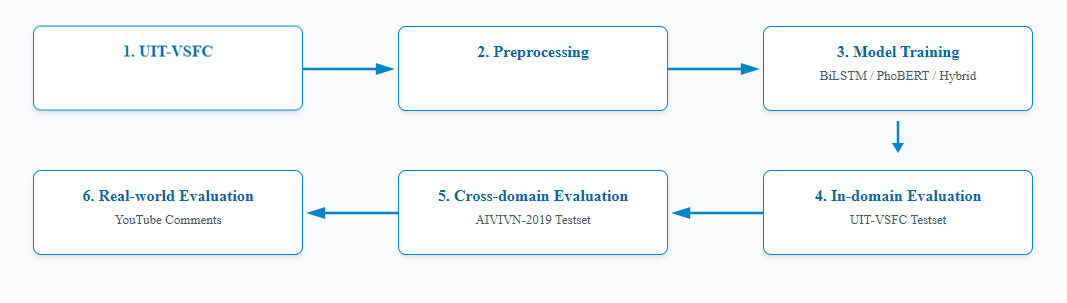
\includegraphics[width=0.9\textwidth]{figures/workflow_diagram.png}
    \caption{The proposed research workflow.}
    \label{fig:workflow}
\end{figure}

\begin{enumerate}
    \item \textbf{Data Acquisition:} Three datasets are used, each serving a distinct purpose in the evaluation design: UIT-VSFC for model training and in-domain validation, AIVIVN-2019 for labeled cross-domain evaluation, and a YouTube comment dataset for real-world, out-of-domain prediction (Section~3.2).
    \item \textbf{Data Preprocessing:} A unified preprocessing pipeline is applied consistently across all three datasets and all three models, ensuring that any observed performance differences are attributable to architectural choices rather than inconsistencies in data handling (Section~3.3).
    \item \textbf{Model Development:} Each of the three architectures --- BiLSTM, PhoBERT, and Hybrid PhoBERT-BiLSTM --- is implemented under a shared binary sentiment classification setting (Positive/Negative), with architecture-specific design choices detailed individually (Section~3.4).
    \item \textbf{Model Training:} All models are trained on the UIT-VSFC training set using architecture-appropriate optimizers and hyperparameters, with early stopping and repeated training across multiple random seeds to ensure statistical reliability of the reported results (Section~3.5).
    \item \textbf{Evaluation:} Trained models are evaluated along two complementary dimensions: (i) predictive performance and efficiency metrics on the in-domain UIT-VSFC test set, and (ii) generalization capability when applied, without retraining, to the out-of-domain AIVIVN-2019 test set and the unlabeled YouTube wild dataset (Sections~3.7--3.8).
\end{enumerate}

Conceptually, the pipeline can be summarized as:
\begin{center}
    \textit{UIT-VSFC} $\rightarrow$ \textit{Preprocessing} $\rightarrow$ \textit{Model Training (BiLSTM / PhoBERT / Hybrid)} $\rightarrow$ \textit{In-domain (UIT-VSFC Testset) Evaluation} $\rightarrow$ \textit{Cross-domain (AIVIVN-2019 Testset) \& Real-world (YouTube Comments) Evaluation}
\end{center}

This design directly operationalizes the four research gaps identified in Section~2.2: applying a single, controlled preprocessing and evaluation pipeline across all three architectures (Gap 1), incorporating a sequence-length-based performance breakdown (Gap 2, detailed in Section~3.3), extending evaluation beyond the training domain through AIVIVN-2019 and YouTube data (Gap 3), and recording training time, inference latency, and model size alongside accuracy metrics (Gap 4, detailed in Section~3.7).

\section{Research Datasets}
\subsection{UIT-VSFC (Training \& Validation)}

The \textbf{UIT-VSFC} (Vietnamese Students' Feedback Corpus) \cite{nguyen2018uitvsfc}, developed by the NLP@UIT research group at the University of Information Technology, VNU-HCM, serves as the primary training and in-domain evaluation resource for this study.

\textbf{Data Collection and Annotation.} The corpus was constructed from real student course-evaluation surveys collected at the end of each semester across three consecutive academic years (2014--2015, 2015--2016, and 2016--2017), yielding over 16,000 raw student responses across 175--227 lecturers and 143--175 subjects per year. Each sentence was independently annotated by multiple human annotators along two dimensions: a three-class \textit{sentiment} label (Positive, Negative, Neutral) and a four-class \textit{topic} label (Lecturer, Curriculum, Facility, Others). Annotation quality was validated using the inter-annotator agreement measure $A_m$ (removing chance agreement), which reached \textbf{91.20\%} for the sentiment task and 71.07\% for the topic task, with observed raw agreement exceeding 95\% and 90\%, respectively --- indicating that sentiment polarity is a substantially less ambiguous annotation target than topic for this corpus.

\textbf{Class Distribution.} The original three-class sentiment distribution is highly imbalanced: Positive accounts for 49.69\%, Negative for 45.99\%, and Neutral for only 4.32\% of the corpus. As established in Section~1.3.1, this study excludes the Neutral class from all training and evaluation, both because of its small and inconsistent representation and because prior work on this corpus reports substantially lower classification performance on Neutral (F1 = 33.99\% with a MaxEnt baseline, versus 91.32\% and 90.52\% for Positive and Negative, respectively) \cite{nguyen2018uitvsfc}, suggesting the label captures linguistically ambiguous or opinion-free sentences rather than a genuine third sentiment polarity.

\textbf{Sentence Length Characteristics.} Feedback sentences in UIT-VSFC are predominantly short: sentences of 1--15 words account for more than 83\% of the corpus, consistent with the informal, single-remark nature of course-evaluation comments. Negative sentences tend to be measurably longer than Positive ones on average, plausibly because expressing dissatisfaction typically requires stating a reason or a suggested improvement. This length characteristic directly motivates the sequence-length-based evaluation strategy adopted in this study (Section~3.3), since a corpus dominated by short sentences may not sufficiently test a model's ability to handle longer-range dependencies.

\textbf{Original Data Split.} The corpus is downloaded via the official data-loading script published by the NLP@UIT research group\footnote{Google Drive-hosted files, retrieved via the official \texttt{VietnameseStudentsFeedback} dataset loader script.}, using a fixed train/validation/test split. Table~\ref{tab:uitvsfc-split} reports the split sizes actually used in this study. Notably, while the Train split size (11,426 sentences) matches the split reported in the original corpus paper \cite{nguyen2018uitvsfc}, the Validation and Test split sizes obtained from the officially distributed download differ from those originally reported (1,538 and 3,166, respectively) --- likely reflecting a later revision of the publicly released files after the original 2018 publication. This study reports and uses the split sizes as actually downloaded and used in all experiments, rather than the originally published figures, to accurately reflect the experimental setup.

\begin{table}[htbp]
    \centering
    \caption{UIT-VSFC train/validation/test split sizes, as actually downloaded and used in this study (sentence-level, all three sentiment classes, prior to Neutral removal).}
    \label{tab:uitvsfc-split}
    \begin{tabular}{lccc}
        \hline
                            & \textbf{Train} & \textbf{Validation} & \textbf{Test} \\
        \hline
        Number of sentences & 11,426         & 3,166               & 1,583         \\
        \hline
    \end{tabular}
\end{table}

\textbf{Class Distribution.} Table~\ref{tab:uitvsfc-train-dist} reports the sentiment class distribution measured directly on the UIT-VSFC training set (11,426 sentences) used in this study. Positive and Negative sentences together account for 95.99\% of the training set, while Neutral represents only 4.01\% --- consistent with the corpus-wide imbalance reported by \cite{nguyen2018uitvsfc}.

\begin{table}[htbp]
    \centering
    \caption{Sentiment class distribution on the UIT-VSFC training set (11,426 sentences).}
    \label{tab:uitvsfc-train-dist}
    \begin{tabular}{lcc}
        \hline
        \textbf{Class} & \textbf{Count}  & \textbf{Proportion (\%)} \\
        \hline
        Positive       & 5,643           & 49.39                    \\
        Negative       & 5,325           & 46.60                    \\
        Neutral        & 458             & 4.01                     \\
        \hline
        \textbf{Total} & \textbf{11,426} & \textbf{100.00}          \\
        \hline
    \end{tabular}
\end{table}

As established in Section~1.3.1, Neutral-labeled sentences are excluded from this study. After this removal, the training set used to fit all three models consists of 10,968 sentences, with a close-to-balanced distribution of 51.45\% Positive and 48.55\% Negative (Table~\ref{tab:uitvsfc-train-binary-dist}), indicating that class imbalance is not a significant concern for the binary classification task adopted in this study.

\begin{table}[htbp]
    \centering
    \caption{Sentiment class distribution on the UIT-VSFC training set after Neutral removal (binary subset used for model training).}
    \label{tab:uitvsfc-train-binary-dist}
    \begin{tabular}{lcc}
        \hline
        \textbf{Class} & \textbf{Count}  & \textbf{Proportion (\%)} \\
        \hline
        Positive       & 5,643           & 51.45                    \\
        Negative       & 5,325           & 48.55                    \\
        \hline
        \textbf{Total} & \textbf{10,968} & \textbf{100.00}          \\
        \hline
    \end{tabular}
\end{table}

\subsection{AIVIVN-2019 (Cross-domain Evaluation)}

The AIVIVN-2019 dataset used for cross-domain evaluation in this study is a community-labeled test set of \textbf{3,217} Vietnamese e-commerce product reviews, derived from the original AIVIVN 2019 Sentiment Analysis Challenge and obtained from a publicly available, community-annotated version shared on Kaggle \cite{aivivn2019kaggle}. Each review is labeled as either Positive or Negative, consistent with the binary scope adopted throughout this study.

\textbf{Sampling for Fair Comparison.} To ensure a fair, size-matched comparison against the in-domain UIT-VSFC test set (Section~3.2.1), rather than evaluating on the full 3,217-review file, a random subsample of size $n = |\text{UIT-VSFC test set}| = 1{,}583$ is drawn from AIVIVN-2019 for each random seed (Section~3.5.4), using that seed to control the sampling. This design choice ensures that observed performance differences between UIT-VSFC and AIVIVN-2019 reflect genuine domain shift rather than differing test-set sizes.

\textbf{Class Distribution.} Table~\ref{tab:aivivn-dist} shows the sentiment class distribution of the full 3,217-review source file (prior to sampling). Positive reviews account for 57.69\%, while Negative reviews account for 42.31\% --- a mild imbalance in the opposite direction compared to UIT-VSFC, but still well within a range that does not require class-balancing techniques.

\begin{table}[htbp]
    \centering
    \caption{Sentiment class distribution on the AIVIVN-2019 test set (3,217 reviews).}
    \label{tab:aivivn-dist}
    \begin{tabular}{lcc}
        \hline
        \textbf{Class} & \textbf{Count} & \textbf{Proportion (\%)} \\
        \hline
        Positive       & 1,856          & 57.69                    \\
        Negative       & 1,361          & 42.31                    \\
        \hline
        \textbf{Total} & \textbf{3,217} & \textbf{100.00}          \\
        \hline
    \end{tabular}
\end{table}

\textbf{Sentence Length Characteristics.} Reviews in AIVIVN-2019 are markedly longer, on average, than UIT-VSFC feedback sentences: the mean length is 20.7 words (median 15, ranging from 1 to 306 words), compared to the predominantly 1--15-word sentences that make up over 83\% of UIT-VSFC. This length gap reflects a genuine domain and register shift --- from short, single-remark course feedback to more elaborate customer reviews --- and constitutes one dimension of the domain generalization challenge investigated in this study.

\textbf{Role in This Study.} As an out-of-domain, differently-registered dataset (informal e-commerce reviews vs.\ semi-formal academic feedback), AIVIVN-2019 is used exclusively for evaluation: all three trained models (BiLSTM, PhoBERT, Hybrid PhoBERT-BiLSTM) are applied to this test set \textit{without any retraining or fine-tuning}, to directly measure cross-domain generalization capability (Section~3.8).

\subsection{YouTube Dataset (Real-world Prediction)}


To evaluate model performance under fully unconstrained, real-world conditions, this study additionally collects and evaluates on a dataset of \textbf{320} Vietnamese comments retrieved via the official YouTube Data API v3 from a single video, ``Những thước phim quý về đại tá, Anh hùng phi công Nguyễn Văn Bảy'' (ANTV), a documentary tribute to a decorated Vietnamese Air Force pilot\footnote{\texttt{https://youtu.be/oFVyyTvHGUo}}. Unlike UIT-VSFC and AIVIVN-2019, this dataset originates from an unmoderated social media context and is expected to exhibit substantially more informal language, including slang, teencode, and inconsistent spelling.

\textbf{Labeling Procedure.} Since YouTube comments carry no ground-truth sentiment label, a hybrid LLM-assisted, human-verified labeling procedure was adopted as a practical alternative to full manual dual-annotation. Figure~\ref{fig:youtube-labeling} illustrates the complete pipeline. Two independently configured Large Language Models (LLMs), accessed via the Groq API, were used as two annotators:
\begin{itemize}
    \item \textbf{Annotator 1:} \texttt{qwen/qwen3-32b}, prompted in English using a system/user role structure with a strict JSON output schema.
    \item \textbf{Annotator 2:} \texttt{LLaMA 3.3 70B}, prompted in Vietnamese using few-shot examples and explicit labeling instructions.
\end{itemize}
Raw comments were first preprocessed (Section~3.3) and then labeled in batches of 8 per request, with each LLM annotator independently assigning one of three labels: \texttt{1} (Positive), \texttt{0} (Negative), or \texttt{-1} (Neutral/Other). Inter-annotator agreement between the two LLMs was measured using Cohen's Kappa. Comments on which the two annotators \textbf{agreed} were retained and passed to a final \textbf{human verification} step, performed by the author, to confirm label correctness. Comments on which the two annotators \textbf{disagreed} (conflict cases) were \textbf{discarded} rather than manually adjudicated, in order to keep only high-confidence, doubly-corroborated labels in the final evaluation set. The resulting fully verified dataset was exported as \texttt{wild\_test\_set\_annotated.csv}, from which the 320-comment binary evaluation subset used in this study (\texttt{-1}/Neutral excluded) was derived.

\begin{figure}[H]
    \centering
    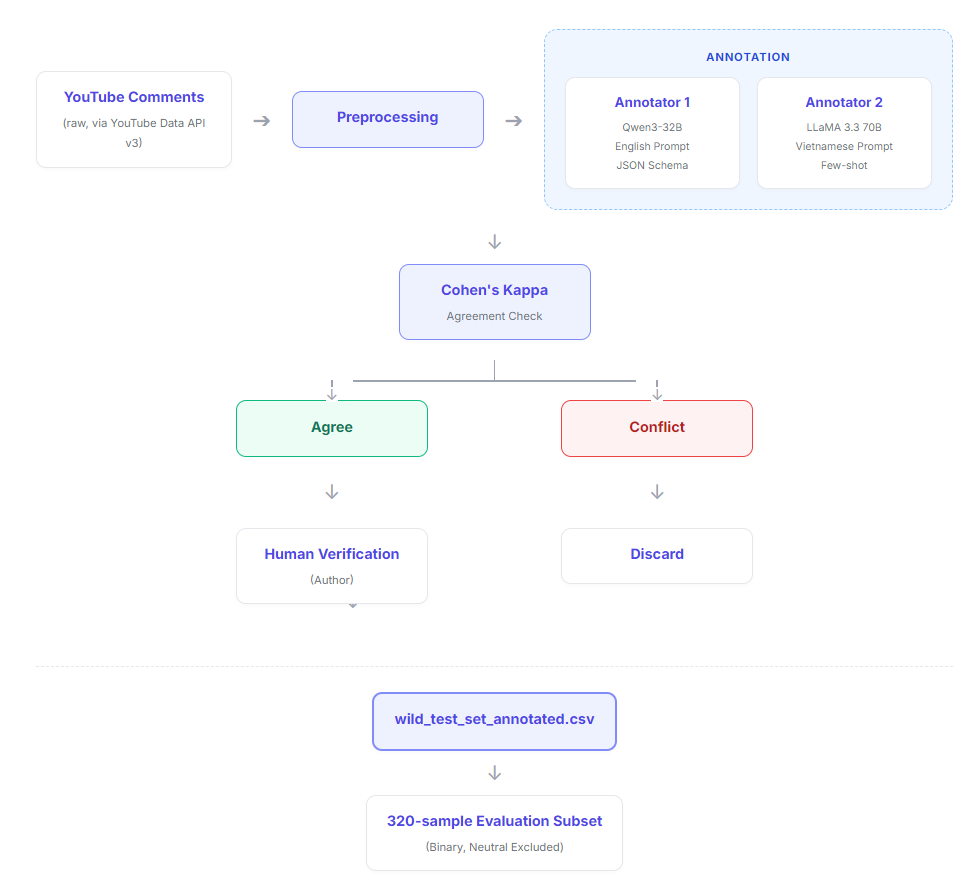
\includegraphics[width=0.7\textwidth]{figures/wild_data_process.png}
    \caption{LLM-assisted, human-verified labeling pipeline for the YouTube wild test set.}
    \label{fig:youtube-labeling}
\end{figure}

\textbf{Class Distribution.} Table~\ref{tab:youtube-dist} shows the resulting sentiment class distribution. Positive comments account for 62.5\%, while Negative comments account for 37.5\% --- the most imbalanced of the three datasets used in this study. This skew is plausibly attributable to the tribute/documentary nature of the source video, which tends to elicit patriotic and appreciative comments, rather than reflecting a general property of YouTube comments.

\begin{table}[htbp]
    \centering
    \caption{Sentiment class distribution on the YouTube wild test set (320 comments).}
    \label{tab:youtube-dist}
    \begin{tabular}{lcc}
        \hline
        \textbf{Class} & \textbf{Count} & \textbf{Proportion (\%)} \\
        \hline
        Positive       & 200            & 62.50                    \\
        Negative       & 120            & 37.50                    \\
        \hline
        \textbf{Total} & \textbf{320}   & \textbf{100.00}          \\
        \hline
    \end{tabular}
\end{table}

\textbf{Sentence Length Characteristics.} Comments in this dataset have a mean length of 22.2 words (median 17, ranging from 5 to 206 words) --- comparable to, and slightly longer than, AIVIVN-2019 reviews, and considerably longer than the predominantly short UIT-VSFC feedback sentences.

\textbf{Role in This Study.} This dataset represents the most challenging generalization scenario in this study: an out-of-domain, unmoderated, informal register that none of the three models have been exposed to during training. As with AIVIVN-2019, all models are applied directly \textit{without retraining}, and the human-verified ground truth enables direct computation of Accuracy and Macro-F1 on this real-world test bed (Section~3.8).


\section{Data Preprocessing}

Because the YouTube wild test set is scraped directly from an unmoderated social media source, it requires an additional, dataset-specific cleaning stage before it can be brought into a common form with UIT-VSFC and AIVIVN-2019. Accordingly, this section is organized into two stages: (i) \textbf{raw text preprocessing}, applied exclusively to the YouTube dataset to remove noise and normalize informal language, and (ii) \textbf{preprocessing for model input}, a unified pipeline applied identically to all three datasets --- UIT-VSFC, AIVIVN-2019, and the now-cleaned YouTube data --- immediately prior to model training or evaluation. This separation ensures that any observed performance differences between BiLSTM, PhoBERT, and Hybrid PhoBERT-BiLSTM are attributable to architectural choices rather than inconsistencies in data handling --- directly addressing Research Gap 1 identified in Section~2.2.

\subsection{Raw Text Preprocessing (YouTube Wild Test Set)}

Raw YouTube comments retrieved via the YouTube Data API v3 are substantially noisier than UIT-VSFC and AIVIVN-2019, which are already curated, research-grade text. UIT-VSFC and AIVIVN-2019 therefore require no processing at this stage; only the YouTube dataset passes through the following pipeline.

\textit{Data Cleaning:}
\begin{enumerate}
    \item Removal of null/NaN entries.
    \item Removal of whitespace-only entries.
    \item Removal of duplicate comments (based on raw content).
    \item Removal of comments containing embedded URLs (regex \texttt{https?://\textbackslash S+|www\textbackslash .\textbackslash S+}), discarded entirely rather than stripped in place, since such comments are frequently spam or promotional content unrelated to genuine sentiment expression.
\end{enumerate}

\textit{Text Normalization (applied sequentially):}
\begin{enumerate}
    \item \textbf{Unicode normalization (NFC).}
    \item \textbf{Timestamp removal:} Patterns of the form \texttt{mm:ss} or \texttt{hh:mm:ss}, commonly used by commenters to reference video moments, are removed.
    \item \textbf{Punctuation normalization:} Repeated punctuation marks are collapsed to a single occurrence (e.g., \texttt{!!!} $\rightarrow$ \texttt{!}).
    \item \textbf{Repeated character normalization:} Characters repeated three or more times are collapsed to two occurrences (e.g., \textit{quáááá} $\rightarrow$ \textit{quáá}), preserving emphasis while removing excessive elongation.
    \item \textbf{Lowercasing.}
    \item \textbf{Teencode replacement:} Vietnamese Internet slang (teencode) is replaced with standard word forms using a teencode dictionary.
    \item \textbf{Special character removal:} Emoticons and special characters are removed, retaining Vietnamese letters, digits, and basic punctuation (\texttt{.}, \texttt{,}, \texttt{!}, \texttt{?}).
    \item \textbf{Whitespace normalization.}
    \item \textbf{Vietnamese text normalization:} Applied via the \texttt{underthesea} library's \texttt{text\_normalize} function.
    \item \textbf{Emoji handling:} Remaining emoji are either converted to their corresponding Vietnamese word or removed.
\end{enumerate}

\textit{Post-processing Filter:}
\begin{enumerate}
    \item Removal of entries left empty after preprocessing.
    \item Removal of comments shorter than 5 words, to exclude content too short to carry reliable sentiment signal.
    \item A final deduplication pass on the cleaned text.
\end{enumerate}

The output of this stage is clean, normalized YouTube comment text, structurally comparable in quality to UIT-VSFC and AIVIVN-2019, and ready to proceed through the unified preprocessing pipeline described in Section~3.3.2.

\subsection{Preprocessing for Model Input}

Starting from this point, an identical pipeline is applied to \textbf{all three datasets} --- UIT-VSFC, AIVIVN-2019, and the cleaned YouTube data (Section~3.3.1) --- to ensure a fair, controlled comparison across domains and across the three models. Prior to this pipeline, sentences originally labeled Neutral (UIT-VSFC) or Neutral/Other (YouTube, Section~3.2.3) are removed, retaining only Positive and Negative examples, consistent with the binary classification scope adopted in Section~1.3.1. The unified pipeline then consists of three steps:

\textbf{Step 1: Text Normalization (\texttt{normalize\_text}).}
\begin{enumerate}
    \item \textbf{Unicode normalization (NFC):} Text is converted to Unicode Normalization Form C, ensuring Vietnamese diacritics are represented as single precomposed characters.
    \item \textbf{Lowercasing:} The entire text is converted to lowercase.
    \item \textbf{Special character removal:} Characters outside the Vietnamese alphabetic range are removed, retaining Vietnamese letters and whitespace only.
    \item \textbf{Whitespace normalization:} Consecutive whitespace characters are collapsed into a single space, and leading/trailing whitespace is stripped.
\end{enumerate}

\textbf{Step 2: Word Segmentation (\texttt{segment\_text}).} Normalized text is segmented into Vietnamese words using \textbf{VnCoreNLP} \cite{vu2018vncorenlp}, accessed via the \texttt{py\_vncorenlp} wrapper, merging multi-syllable compound words into single tokens (e.g., \textit{sinh viên} $\rightarrow$ \textit{sinh\_viên}, meaning ``student''). This step is necessary because Vietnamese word boundaries do not align with whitespace.

\textbf{Step 3: Tokenization.} The segmented text is converted into a numerical representation in an architecture-specific manner:
\begin{itemize}
    \item \textbf{BiLSTM:} A custom word-level tokenizer, fit exclusively on the segmented UIT-VSFC training set, is used to convert sentences to integer sequences (\texttt{texts\_to\_sequences}), followed by fixed-length padding/truncation (\texttt{pad\_sequences}).
    \item \textbf{PhoBERT and Hybrid PhoBERT-BiLSTM:} The pretrained HuggingFace tokenizer bundled with \texttt{vinai/phobert-base} \cite{nguyen2020phobert} is used directly, ensuring full compatibility with PhoBERT's pretrained subword vocabulary.
\end{itemize}

\section{Proposed Models}

This study implements and compares three deep learning architectures for binary Vietnamese sentiment classification (Positive/Negative): a BiLSTM baseline, a fine-tuned PhoBERT baseline, and a proposed Hybrid PhoBERT-BiLSTM architecture. All three models share the same binary classification output space but differ substantially in how they represent and process input text.

\subsection{BiLSTM Architecture}

The BiLSTM model serves as a lightweight, non-pretrained baseline. As illustrated in Figure~\ref{fig:bilstm-arch}, the architecture consists of a randomly initialized, trainable embedding layer, followed by a single bidirectional LSTM layer and a stack of dropout regularization layers before the final classification head:
\begin{itemize}
    \item \textbf{Embedding Layer:} Randomly initialized (not pretrained), trainable during training, mapping each token index to a dense vector.
    \item \textbf{Dropout (0.3):} Applied to the embedded sequence.
    \item \textbf{Bidirectional LSTM (hidden size = 64):} Processes the sequence in both directions, capturing context from preceding and following tokens.
    \item \textbf{Dropout (0.6) and Dropout (0.5):} Two successive dropout layers applied after the recurrent layer for regularization.
    \item \textbf{Fully Connected Layer (64 $\rightarrow$ 2):} Maps the final representation to the two output classes.
\end{itemize}
Because this model relies entirely on randomly initialized embeddings, without any pretrained linguistic knowledge, it represents the performance achievable by a standard recurrent architecture trained \textit{from scratch} on UIT-VSFC alone.

\begin{figure}[htbp]
    \centering
    \begin{tikzpicture}[
        box/.style={rectangle, draw, rounded corners, minimum width=4.2cm, minimum height=0.9cm, align=center, font=\small},
        arr/.style={-{Stealth[length=2mm]}, thick},
        node distance=0.5cm
        ]
        \node[box, fill=blue!8]  (input)  {Input\\(padded word-index sequence)};
        \node[box, fill=green!8, below=of input]  (emb)    {Embedding Layer\\(random init, trainable)};
        \node[box, below=of emb]  (drop1)  {Dropout (0.3)};
        \node[box, fill=orange!12, below=of drop1] (lstm)   {Bidirectional LSTM\\(hidden size = 64)};
        \node[box, below=of lstm] (drop2)  {Dropout (0.6)};
        \node[box, below=of drop2] (drop3)  {Dropout (0.5)};
        \node[box, fill=purple!10, below=of drop3] (fc)     {Fully Connected (64 $\rightarrow$ 2)};
        \node[box, fill=blue!8, below=of fc]  (out)    {Output\\(Positive / Negative)};
        \draw[arr] (input) -- (emb);
        \draw[arr] (emb) -- (drop1);
        \draw[arr] (drop1) -- (lstm);
        \draw[arr] (lstm) -- (drop2);
        \draw[arr] (drop2) -- (drop3);
        \draw[arr] (drop3) -- (fc);
        \draw[arr] (fc) -- (out);
    \end{tikzpicture}
    \caption{BiLSTM model architecture.}
    \label{fig:bilstm-arch}
\end{figure}

\subsection{PhoBERT Architecture}

The PhoBERT baseline uses \texttt{vinai/phobert-base} \cite{nguyen2020phobert}, a monolingual Transformer encoder pretrained on 20GB of Vietnamese text, fine-tuned end-to-end (all parameters trainable) via HuggingFace's \texttt{AutoModelForSequenceClassification}. As shown in Figure~\ref{fig:phobert-arch}, input text is tokenized using PhoBERT's native Byte-Pair Encoding (BPE) tokenizer, encoded through all 12 Transformer layers, and the final-layer representation of the special \texttt{[CLS]} token is passed through a classification head to produce the Positive/Negative prediction. Unlike the BiLSTM and Hybrid models, PhoBERT is fully fine-tuned rather than frozen, allowing all pretrained weights to be updated during training.

\begin{figure}[htbp]
    \centering
    \begin{tikzpicture}[
        box/.style={rectangle, draw, rounded corners, minimum width=4.6cm, minimum height=0.9cm, align=center, font=\small},
        arr/.style={-{Stealth[length=2mm]}, thick},
        node distance=0.5cm
        ]
        \node[box, fill=blue!8]  (input)  {Input\\(BPE tokens)};
        \node[box, fill=orange!12, below=of input]  (phobert) {vinai/phobert-base\\(12 layers, fully fine-tuned)};
        \node[box, fill=green!8, below=of phobert]  (cls)    {\texttt{[CLS]} token embedding};
        \node[box, fill=purple!10, below=of cls]  (head)   {Classification Head};
        \node[box, fill=blue!8, below=of head]  (out)    {Output\\(Positive / Negative)};
        \draw[arr] (input) -- (phobert);
        \draw[arr] (phobert) -- (cls);
        \draw[arr] (cls) -- (head);
        \draw[arr] (head) -- (out);
    \end{tikzpicture}
    \caption{PhoBERT model architecture.}
    \label{fig:phobert-arch}
\end{figure}

\subsection{Proposed Hybrid PhoBERT-BiLSTM Architecture}

The Hybrid model is designed to combine PhoBERT's contextual embedding power with the sequential feature extraction of a BiLSTM layer, while substantially reducing computational cost relative to full PhoBERT fine-tuning. As illustrated in Figure~\ref{fig:hybrid-arch}, this architecture makes three key design choices that distinguish it from a straightforward PhoBERT+BiLSTM stack:

\begin{itemize}
    \item \textbf{Truncated PhoBERT Encoder:} Rather than using the full 12-layer PhoBERT-base encoder, only the first \textbf{8 of 12} Transformer layers are retained (\texttt{encoder.layer[:8]}); the remaining 4 layers are discarded. This reduces the computational cost of the forward pass through the pretrained encoder while retaining its lower- and mid-level contextual representations.
    \item \textbf{Frozen Feature Extraction:} All parameters of the (truncated) PhoBERT encoder are frozen (\texttt{requires\_grad=False}); PhoBERT is used purely as a static feature extractor and is not updated during training. Only the BiLSTM and final classification layers are trained.
    \item \textbf{Full-Sequence Input to BiLSTM:} Rather than using only the \texttt{[CLS]} token embedding (as in the PhoBERT baseline), the \textbf{entire sequence} of final-layer hidden states (\texttt{last\_hidden\_state}, shape: batch $\times$ sequence length $\times$ 768) is passed into the BiLSTM layer, allowing the recurrent layer to model sequential dependencies across all token representations rather than relying on a single pooled vector.
\end{itemize}

The full forward pass proceeds as follows: token sequences are encoded by the truncated, frozen PhoBERT encoder; the resulting sequence of hidden states passes through a Dropout layer (rate 0.1); a single bidirectional LSTM layer (hidden size = 256) processes the sequence; the final forward and backward hidden states are concatenated (dimension 512); and a fully connected layer (512 $\rightarrow$ 2) produces the final classification logits.

\begin{figure}[htbp]
    \centering
    \begin{tikzpicture}[
        box/.style={rectangle, draw, rounded corners, minimum width=5.2cm, minimum height=0.9cm, align=center, font=\small},
        arr/.style={-{Stealth[length=2mm]}, thick},
        node distance=0.5cm
        ]
        \node[box, fill=blue!8]  (input)  {Input\\(BPE tokens)};
        \node[box, fill=red!10, below=of input]  (phobert) {vinai/phobert-base\\\textbf{(8 of 12 layers, FROZEN)}};
        \node[box, fill=green!8, below=of phobert]  (seq)    {\texttt{last\_hidden\_state}\\(full sequence, 768-dim per token)};
        \node[box, below=of seq]  (drop)   {Dropout (0.1)};
        \node[box, fill=orange!12, below=of drop]  (bilstm) {Bidirectional LSTM\\(hidden size = 256)};
        \node[box, fill=green!8, below=of bilstm]  (concat) {Concat final hidden states\\(forward + backward, dim = 512)};
        \node[box, fill=purple!10, below=of concat]  (fc)     {Fully Connected (512 $\rightarrow$ 2)};
        \node[box, fill=blue!8, below=of fc]  (out)    {Output\\(Positive / Negative)};
        \draw[arr] (input) -- (phobert);
        \draw[arr] (phobert) -- (seq);
        \draw[arr] (seq) -- (drop);
        \draw[arr] (drop) -- (bilstm);
        \draw[arr] (bilstm) -- (concat);
        \draw[arr] (concat) -- (fc);
        \draw[arr] (fc) -- (out);
    \end{tikzpicture}
    \caption{Proposed Hybrid PhoBERT-BiLSTM architecture, using a truncated (8-layer), frozen PhoBERT encoder.}
    \label{fig:hybrid-arch}
\end{figure}

\section{Model Training}

\subsection{Training Pipeline}
All three models are trained on the UIT-VSFC training set (Section~3.2.1) following the preprocessing pipeline described in Section~3.3. Each model is trained independently, with model-specific optimizers, learning rates, and training durations, but a shared evaluation protocol: validation performance (Macro-F1) is monitored after every epoch, the best-performing checkpoint is retained (\texttt{load\_best\_model\_at\_end} for PhoBERT and Hybrid), and training is stopped early if validation performance fails to improve.

\subsection{Hyperparameters and Optimizer}

\textbf{BiLSTM.} Trained using the Adam optimizer \cite{kingma2014adam} with a learning rate of $1\times10^{-3}$ and weight decay of $1\times10^{-4}$, batch size 32.

\textbf{PhoBERT.} Fine-tuned end-to-end using AdamW \cite{loshchilov2019adamw} (via the HuggingFace \texttt{Trainer} API \cite{wolf2020transformers}) with a learning rate of $2\times10^{-5}$, batch size 32, and mixed-precision (fp16) training enabled on GPUs supporting it (compute capability $\geq$ 7.0).

\textbf{Hybrid PhoBERT-BiLSTM.} Since the (truncated) PhoBERT encoder is entirely frozen, only the BiLSTM and fully connected layers are optimized. A custom AdamW \cite{loshchilov2019adamw} optimizer is constructed with parameter groups restricted to these trainable components, using a learning rate of $1\times10^{-3}$ for both the BiLSTM and the fully connected layer; PhoBERT's parameters are excluded from the optimizer entirely, as they carry no gradient. Weight decay is set to the HuggingFace \texttt{Trainer} \cite{wolf2020transformers} default of $0.01$.

Table~\ref{tab:training-hyperparams} summarizes the training configuration for all three models.

\begin{table}[htbp]
    \centering
    \caption{Training hyperparameters for BiLSTM, PhoBERT, and Hybrid PhoBERT-BiLSTM.}
    \label{tab:training-hyperparams}
    \begin{tabular}{lccc}
        \hline
                                & \textbf{BiLSTM}  & \textbf{PhoBERT}   & \textbf{Hybrid}                      \\
        \hline
        Optimizer               & Adam             & AdamW              & AdamW (custom groups)                \\
        Learning rate           & $1\times10^{-3}$ & $2\times10^{-5}$   & $1\times10^{-3}$ (BiLSTM \& FC only) \\
        Weight decay            & $1\times10^{-4}$ & 0.01               & 0.01                                 \\
        Batch size              & 32               & 32                 & 32                                   \\
        Max epochs              & 15               & 5                  & 15                                   \\
        Early stopping patience & 3                & 3                  & 3                                    \\
        Mixed precision (fp16)  & ---              & Yes (if supported) & ---                                  \\
        \hline
    \end{tabular}
\end{table}

\subsection{Early Stopping}
For PhoBERT and Hybrid PhoBERT-BiLSTM, training employs the HuggingFace \texttt{Trainer}'s \cite{wolf2020transformers} \texttt{EarlyStoppingCallback}, which halts training if the validation Macro-F1 score fails to improve by at least $0.001$ over a window of 3 consecutive evaluation epochs (\texttt{early\_stopping\_patience=3}, \texttt{early\_stopping\_threshold=0.001}). Combined with \texttt{load\_best\_model\_at\_end=True}, this ensures that the checkpoint ultimately retained for evaluation corresponds to the epoch with the best validation Macro-F1, rather than the final training epoch.

\subsection{Multiple Random Seeds}
To account for the sensitivity of deep learning models to weight initialization and training randomness, each of the three models is trained independently \textbf{five times}, using a fixed set of random seeds: $\{42, 0, 1, 123, 2026\}$. For each seed, a freshly initialized model is trained from scratch (avoiding any weight leakage between runs), and all stochastic components --- including CPU, NumPy, and (where applicable) CUDA random number generators --- are seeded identically. Training runs are logged individually to Weights \& Biases (W\&B) \cite{wandb} for experiment tracking, and results across the five seeds are aggregated (mean and standard deviation) when reporting final performance in Chapter~4.

\section{Experimental Configuration}

\subsection{Hardware}
All experiments in this study --- training of the BiLSTM, PhoBERT, and Hybrid PhoBERT-BiLSTM models, across five random seeds each --- were conducted on \textbf{Google Colab}\footnote{\url{https://colab.research.google.com/}} (free tier), using a single \textbf{NVIDIA Tesla T4} GPU (16GB VRAM) per session.

\subsection{Software}
All models were implemented in \textbf{Python}, using \textbf{PyTorch} \cite{paszke2019pytorch} as the primary deep learning framework, installed via the CUDA 11.8-compatible wheel distribution. PhoBERT and Hybrid PhoBERT-BiLSTM additionally rely on the HuggingFace \texttt{transformers} library \cite{wolf2020transformers} (installed from the latest GitHub source at the time of experimentation) for pretrained model loading, tokenization, and the \texttt{Trainer} training loop. Vietnamese word segmentation is performed via \texttt{py-vncorenlp} \cite{vu2018vncorenlp}. Experiment tracking and logging are handled through Weights \& Biases (\texttt{wandb}) \cite{wandb}. Additional supporting libraries include \texttt{gdown} (dataset retrieval) and \texttt{torchinfo} (model summary inspection).

\subsection{Development Environment}
All notebooks were developed and executed within the \textbf{Google Colab} notebook environment, which provides on-demand GPU access, persistent Google Drive integration for dataset and checkpoint storage, and native support for the package installation workflow (\texttt{!pip install}) used throughout this study.

\section{Evaluation Methodology}

Model performance is assessed along two complementary dimensions: \textbf{predictive quality} (how accurately each model classifies sentiment, following standard classification evaluation practice \cite{sokolova2009systematic}) and \textbf{computational efficiency} (how costly each model is to train and deploy). Reporting both dimensions directly addresses Research Gap 4 identified in Section~2.2, which highlights the general neglect of deployment-related trade-offs in prior Vietnamese sentiment analysis literature.

\subsection{Predictive Performance Metrics}

For the binary classification setting adopted in this study, predictions are evaluated using the following standard metrics, computed with Positive as the reference class unless otherwise noted:

\begin{align}
    \text{Accuracy}  & = \frac{TP + TN}{TP + TN + FP + FN}                                                       \\
    \text{Precision} & = \frac{TP}{TP + FP}                                                                      \\
    \text{Recall}    & = \frac{TP}{TP + FN}                                                                      \\
    F_1              & = 2 \times \frac{\text{Precision} \times \text{Recall}}{\text{Precision} + \text{Recall}}
\end{align}

Since predictions must be interpretable for both Positive and Negative classes, \textbf{Macro-F1} --- the unweighted average of the per-class $F_1$ scores --- is used as the primary metric for model selection (early stopping and checkpoint selection, Section~3.5) and for cross-model comparison in Chapter~4, as it treats both classes equally regardless of their relative frequency in each dataset (Section~3.2). Precision, Recall, and per-class $F_1$ are additionally reported to support finer-grained error analysis. A \textbf{confusion matrix} is generated for each model on a fixed 300-sample subset of each test set (size-matched for comparability across UIT-VSFC, AIVIVN-2019, and the YouTube wild test set), enabling inspection of the specific distribution of correct predictions, false positives, and false negatives.

\subsection{Computational Efficiency Metrics}

To characterize the practical deployment cost of each architecture, three additional metrics are recorded:

\begin{itemize}
    \item \textbf{Training Time:} Wall-clock time elapsed during model training, measured via Python's \texttt{time} module around the training loop of each run.
    \item \textbf{Inference Latency:} Average per-sample inference time, measured separately on \textbf{CPU} and \textbf{GPU}. For each device, the trained model is set to evaluation mode, a batch of representative input samples is tokenized, and inference is executed for \textbf{10 runs} using \texttt{time.perf\_counter()} (CPU) or the CUDA-synchronized equivalent (GPU); the reported latency is the mean elapsed time across these 10 runs, expressed in milliseconds.
    \item \textbf{Model Size / Parameters:} The total number of model parameters, as well as the number of \textit{trainable} parameters, is computed directly from the underlying PyTorch model (\texttt{sum(p.numel() for p in model.parameters())}, with an additional filter on \texttt{requires\_grad} for the trainable count). This distinction is particularly relevant for the Hybrid PhoBERT-BiLSTM model, where a substantial fraction of total parameters (the frozen, truncated PhoBERT encoder) are non-trainable.
\end{itemize}

These efficiency metrics are reported alongside predictive performance in Chapter~4, enabling a direct accuracy-versus-cost comparison across the three architectures --- a comparison largely absent from prior Vietnamese sentiment analysis studies (Section~2.2).

\section{Cross-domain Evaluation Strategy}

To assess not only in-domain predictive performance but also the ability of each model to generalize beyond its training distribution, this study evaluates all three trained models --- BiLSTM, PhoBERT, and Hybrid PhoBERT-BiLSTM --- on three test sets of increasing distributional distance from the training domain, \textit{without any retraining or fine-tuning} on any of them. This design directly targets Research Gap 3 identified in Section~2.2: the general lack of domain generalization assessment in prior Vietnamese sentiment analysis studies.

\subsection{Evaluation on UIT-VSFC (In-domain)}
Each model is first evaluated on the official UIT-VSFC test set (Section~3.2.1, Table~\ref{tab:uitvsfc-split}), after Neutral-label removal. As this test set is drawn from the same distribution as the training data (same source, register, and annotation guidelines), this evaluation establishes each model's \textbf{in-domain, upper-bound performance}, serving as the reference point against which generalization degradation on the two out-of-domain test sets is measured.

\subsection{Evaluation on AIVIVN-2019 (Cross-domain)}
Each model is then evaluated, without retraining, on the AIVIVN-2019 test set (Section~3.2.2): 3,217 Vietnamese e-commerce product reviews, labeled Positive/Negative. This dataset differs from UIT-VSFC along two dimensions simultaneously --- \textit{domain} (educational feedback vs.\ product reviews) and \textit{register} (short, semi-formal remarks vs.\ longer, more elaborate consumer language, as established in Section~3.2.2) --- providing a controlled test of cross-domain generalization under a labeled, verifiable ground truth.

\subsection{Prediction on YouTube Comments (Real-world, Out-of-domain)}
Finally, each model is applied, without retraining, to the 320-comment YouTube wild test set (Section~3.2.3), constructed via the LLM-assisted, human-verified labeling procedure described in Section~3.2.3. This dataset represents the most challenging generalization scenario examined in this study: fully unmoderated, informal social media text, potentially containing slang, teencode, and irregular spelling not represented in either training domain.

\subsection{Comparative Analysis}
For each of the three test sets, Accuracy, Precision, Recall, and Macro-F1 (Section~3.7) are computed for every model, together with a confusion matrix on a fixed 300-sample subset (size-matched for comparability across UIT-VSFC, AIVIVN-2019, and the YouTube wild test set) and a breakdown by sentence-length category (Short/Medium/Long, using the fixed thresholds established in Section~3.3.2). Comparing performance across the three test sets --- rather than reporting a single aggregate score --- allows this study to directly quantify each architecture's \textit{domain generalization gap}: the drop in Macro-F1 from the in-domain UIT-VSFC test set to each out-of-domain test set. This comparative analysis, presented in full in Chapter~4, is designed to reveal whether architectural complexity (e.g., PhoBERT's pretrained contextual representations) translates into more robust cross-domain generalization, or whether all three models degrade similarly when applied outside their training distribution.
\section{Chapter Summary}

This chapter has presented the complete research methodology underlying this thesis. Section~3.1 outlined the overall five-stage research pipeline, from data acquisition through cross-domain evaluation. Section~3.2 described the three datasets used --- UIT-VSFC for training and in-domain evaluation, AIVIVN-2019 for labeled cross-domain evaluation, and a YouTube wild test set, LLM-labeled and human-verified, for real-world evaluation --- together with their class distributions and sentence-length characteristics. Section~3.3 detailed the two-stage preprocessing pipeline: dataset-specific raw text cleaning for the noisy YouTube data, followed by a unified normalization, word-segmentation, and tokenization pipeline applied identically across all three datasets and all three models. Section~3.4 presented the three model architectures compared in this study --- BiLSTM, PhoBERT, and the proposed Hybrid PhoBERT-BiLSTM, the latter using a truncated (8-of-12-layer), frozen PhoBERT encoder combined with a trainable bidirectional LSTM. Section~3.5 described the model-specific training procedures, including optimizers, learning rates, early stopping, and repeated training across five random seeds to ensure statistically reliable results. Section~3.6 documented the hardware, software, and development environment used throughout. Section~3.7 defined the evaluation metrics employed, spanning both predictive performance (Accuracy, Precision, Recall, Macro-F1) and computational efficiency (training time, inference latency, model size). Finally, Section~3.8 described the cross-domain evaluation strategy, under which all three trained models are applied, without retraining, to the in-domain UIT-VSFC test set and to two out-of-domain test sets of increasing distributional distance, in order to directly measure domain generalization capability.

Together, these methodological choices are designed to enable a controlled, reproducible, and generalization-aware comparison of BiLSTM, PhoBERT, and Hybrid PhoBERT-BiLSTM --- directly addressing the four research gaps identified in Section~2.2. Chapter~4 presents the experimental results obtained under this methodology.

\chapter{Experimental Results}

This chapter presents the complete experimental results and quantitative evaluation of the three models --- BiLSTM, PhoBERT, and Hybrid PhoBERT-BiLSTM --- following the methodology described in Chapter~3.

\section{Experimental Setup}

\subsection{Experimental Environment}
All experiments were conducted on \textbf{Google Colab} (free tier), using a single \textbf{NVIDIA Tesla T4} GPU (16GB VRAM), as detailed in Section~3.6. Models were implemented in \textbf{PyTorch} \cite{paszke2019pytorch}, with PhoBERT and Hybrid PhoBERT-BiLSTM additionally relying on the HuggingFace \texttt{transformers} library \cite{wolf2020transformers}.

\subsection{Dataset Splitting Strategy}
Models are trained on the UIT-VSFC training split (10,968 sentences after Neutral removal, Section~3.2.1) and validated on the UIT-VSFC validation split, both used exactly as officially distributed, without re-partitioning. Final evaluation is conducted on three test sets of increasing distributional distance from the training domain: the officially distributed UIT-VSFC test split (1,583 sentences, in-domain), a size-matched random subsample of AIVIVN-2019 ($n = 1{,}583$, cross-domain, resampled per seed as described in Section~3.2.2), and the full YouTube wild test set (320 comments, real-world out-of-domain), as described in Sections~3.2.1--3.2.3.
\subsection{Evaluation Protocol}
Consistent with Section~3.8, each trained model is evaluated on all three test sets \textit{without any retraining or fine-tuning} between test sets. For every (model, seed, test set) combination, Accuracy and Macro-F1 are computed overall, as well as broken down by sentence-length category (Short/Medium/Long, Section~3.3.2). Domain generalization is quantified via the relative drop in Accuracy and Macro-F1 from the in-domain UIT-VSFC result to each out-of-domain result.

\subsection{Hyperparameter Settings}
Model-specific hyperparameters --- optimizer, learning rate, weight decay, batch size, maximum epochs, and early stopping configuration --- follow exactly the settings established in Section~3.5 (Table~\ref{tab:training-hyperparams}) and are not repeated here.

\subsection{Random Seed Configuration}
As established in Section~3.5, each of the three models is trained independently five times, using the fixed seed set $\{42, 0, 1, 123, 2026\}$, yielding 15 trained model instances in total. All results reported in this chapter are aggregated across these five seeds (mean $\pm$ standard deviation), unless otherwise specified.

\section{Performance Evaluation on UIT-VSFC}

\subsection{Overall Classification Results}
Table~\ref{tab:uitvsfc-results} reports Accuracy and Macro-F1 for all three models on the in-domain UIT-VSFC test set, aggregated across five random seeds (mean $\pm$ standard deviation).

\begin{table}[htbp]
    \centering
    \caption{Overall classification performance on the UIT-VSFC test set (in-domain), mean $\pm$ standard deviation across 5 seeds.}
    \label{tab:uitvsfc-results}
    \begin{tabular}{lcc}
        \hline
        \textbf{Model}        & \textbf{Accuracy (\%)}    & \textbf{Macro-F1 (\%)}    \\
        \hline
        BiLSTM                & $95.20 \pm 0.69$          & $95.17 \pm 0.68$          \\
        PhoBERT               & $\mathbf{98.20 \pm 0.30}$ & $\mathbf{98.19 \pm 0.30}$ \\
        Hybrid PhoBERT-BiLSTM & $97.60 \pm 0.55$          & $97.58 \pm 0.56$          \\
        \hline
    \end{tabular}
\end{table}

PhoBERT achieves the highest in-domain performance, with the lowest variance across seeds (std $= 0.30$), indicating both superior accuracy and greater training stability compared to the other two architectures. The Hybrid PhoBERT-BiLSTM model, despite using only a truncated, frozen 8-layer PhoBERT encoder, closely approaches full PhoBERT's performance (within 0.6 percentage points of Accuracy), while BiLSTM trails both pretrained-based models by approximately 2.4--3.0 percentage points, consistent with its reliance on randomly initialized embeddings rather than pretrained contextual representations (Section~3.4.1).

\subsection{Confusion Matrix}
Table~\ref{tab:confmat-uitvsfc} presents the confusion matrix for each model's \textbf{best-performing seed} (by UIT-VSFC Macro-F1: BiLSTM seed 2026, PhoBERT seed 2026, Hybrid PhoBERT-BiLSTM seed 123), evaluated on the corresponding 300-sample subset of the UIT-VSFC test set, reconstructed from the classification report precision/recall/support values.

\begin{table}[htbp]
    \centering
    \caption{Confusion matrix on the UIT-VSFC test set (300-sample subset, best seed per model).}
    \label{tab:confmat-uitvsfc}
    \begin{tabular}{llcc}
        \hline
        \textbf{Model}                                    &                 & \textbf{Predicted Negative} & \textbf{Predicted Positive} \\
        \hline
        \multirow{2}{*}{BiLSTM (seed 2026)}               & Actual Negative & 132                         & 5                           \\
                                                          & Actual Positive & 7                           & 156                         \\
        \hline
        \multirow{2}{*}{PhoBERT (seed 2026)}              & Actual Negative & 135                         & 2                           \\
                                                          & Actual Positive & 2                           & 161                         \\
        \hline
        \multirow{2}{*}{Hybrid PhoBERT-BiLSTM (seed 123)} & Actual Negative & 141                         & 3                           \\
                                                          & Actual Positive & 2                           & 154                         \\
        \hline
    \end{tabular}
\end{table}

At their respective best seeds, PhoBERT achieves the most balanced error distribution (2 false positives, 2 false negatives out of 300), while Hybrid PhoBERT-BiLSTM makes slightly more false positives (3) but fewer false negatives (2), and BiLSTM makes the most errors overall (12 total misclassifications, versus 4 for PhoBERT and 5 for Hybrid). This is consistent with the overall Macro-F1 ranking established in Table~\ref{tab:uitvsfc-results}, and further confirms that the pretrained-representation models (PhoBERT and Hybrid) generalize more reliably than the from-scratch BiLSTM even under favorable random initialization.

\subsection{Comparison among BiLSTM, PhoBERT, and Hybrid PhoBERT-BiLSTM}
Ranking all three models by in-domain Macro-F1 yields: PhoBERT (98.19\%) $>$ Hybrid PhoBERT-BiLSTM (97.58\%) $>$ BiLSTM (95.17\%). This ordering confirms that pretrained contextual representations (PhoBERT, Hybrid) provide a measurable advantage over embeddings learned from scratch (BiLSTM) on the in-domain task, even when, as in the Hybrid model, the pretrained encoder is truncated to 8 layers and entirely frozen (Section~3.4.3). The relatively small gap between PhoBERT and Hybrid (0.61 percentage points in Macro-F1) suggests that most of PhoBERT's in-domain representational benefit is retained even under this reduced-computation configuration --- a trade-off examined further in terms of computational cost in Section~4.5.


\section{Cross-domain Evaluation on AIVIVN-2019}

\subsection{Performance on Unseen Domain}
Table~\ref{tab:aivivn-results} reports Accuracy and Macro-F1 for all three models on the AIVIVN-2019 test set (Section~3.2.2), applied \textit{without any retraining}, aggregated across five random seeds.

\begin{table}[htbp]
    \centering
    \caption{Cross-domain classification performance on AIVIVN-2019, mean $\pm$ standard deviation across 5 seeds.}
    \label{tab:aivivn-results}
    \begin{tabular}{lcc}
        \hline
        \textbf{Model}        & \textbf{Accuracy (\%)}    & \textbf{Macro-F1 (\%)}    \\
        \hline
        BiLSTM                & $70.40 \pm 2.82$          & $70.33 \pm 2.83$          \\
        PhoBERT               & $\mathbf{83.73 \pm 1.69}$ & $\mathbf{83.63 \pm 1.59}$ \\
        Hybrid PhoBERT-BiLSTM & $79.87 \pm 4.23$          & $79.81 \pm 4.23$          \\
        \hline
    \end{tabular}
\end{table}

\subsection{Comparison with In-domain Results}
Table~\ref{tab:indomain-vs-aivivn} juxtaposes in-domain (UIT-VSFC, Table~\ref{tab:uitvsfc-results}) and cross-domain (AIVIVN-2019) Macro-F1 for all three models.

\begin{table}[htbp]
    \centering
    \caption{In-domain vs.\ cross-domain (AIVIVN-2019) Macro-F1 comparison.}
    \label{tab:indomain-vs-aivivn}
    \begin{tabular}{lccc}
        \hline
        \textbf{Model}        & \textbf{UIT-VSFC F1 (\%)} & \textbf{AIVIVN-2019 F1 (\%)} & \textbf{Absolute Gap (pp)} \\
        \hline
        BiLSTM                & 95.17                     & 70.33                        & 24.84                      \\
        PhoBERT               & 98.19                     & 83.63                        & 14.56                      \\
        Hybrid PhoBERT-BiLSTM & 97.58                     & 79.81                        & 17.77                      \\
        \hline
    \end{tabular}
\end{table}

While PhoBERT and Hybrid PhoBERT-BiLSTM maintain a substantial performance advantage over BiLSTM in-domain (Section~4.2), this advantage becomes markedly larger under cross-domain evaluation: PhoBERT outperforms BiLSTM by 13.33 percentage points on AIVIVN-2019 (83.63\% vs.\ 70.33\% Macro-F1), compared to only 3.02 percentage points in-domain. This indicates that PhoBERT's pretrained contextual representations provide most of their practical benefit precisely in the out-of-domain setting, where BiLSTM's randomly initialized, UIT-VSFC-specific embeddings fail to transfer.

\subsection{Generalization Capability}
Ranking the three models by absolute Macro-F1 gap between in-domain and cross-domain performance (smaller gap indicating better generalization) yields: PhoBERT (14.56 pp) $<$ Hybrid PhoBERT-BiLSTM (17.77 pp) $<$ BiLSTM (24.84 pp). PhoBERT generalizes best despite (or arguably because of) being fully fine-tuned on UIT-VSFC, suggesting that its pretrained linguistic knowledge, acquired from 20GB of general-domain Vietnamese text \cite{nguyen2020phobert}, is not overwritten during fine-tuning to the extent that it loses transferability. The Hybrid model, despite using a frozen, truncated (8-layer) PhoBERT encoder, retains a meaningfully smaller generalization gap than BiLSTM, indicating that even a reduced, non-fine-tuned pretrained representation transfers better than embeddings learned entirely from the training domain.

\subsection{Performance Degradation Analysis}
Table~\ref{tab:degradation-aivivn} reports the relative performance drop (\%) from in-domain UIT-VSFC to AIVIVN-2019, computed per seed as $(F1_{\text{UIT-VSFC}} - F1_{\text{AIVIVN}}) / F1_{\text{UIT-VSFC}}$ and aggregated across the five seeds.

\begin{table}[htbp]
    \centering
    \caption{Relative Macro-F1 degradation (\%) from UIT-VSFC to AIVIVN-2019, mean $\pm$ standard deviation across 5 seeds.}
    \label{tab:degradation-aivivn}
    \begin{tabular}{lc}
        \hline
        \textbf{Model}        & \textbf{Macro-F1 Drop (\%)} \\
        \hline
        BiLSTM                & $24.83 \pm 2.29$            \\
        PhoBERT               & $\mathbf{14.56 \pm 1.18}$   \\
        Hybrid PhoBERT-BiLSTM & $17.77 \pm 3.44$            \\
        \hline
    \end{tabular}
\end{table}

Beyond having the lowest mean degradation, PhoBERT also exhibits the lowest variance across seeds (std $= 1.18$), indicating that its cross-domain robustness is consistent rather than dependent on a favorable random initialization. In contrast, the Hybrid model shows the highest variance (std $= 3.44$) among the three, suggesting that its cross-domain generalization is comparatively more sensitive to training randomness, despite outperforming BiLSTM on average.

\section{Sequence Length Analysis}

\subsection{Sentence Length Distribution}
Following the fixed Short/Medium/Long thresholds established in Section~3.3.2 (derived from the 33rd/66th percentiles of the UIT-VSFC training set), Table~\ref{tab:length-dist} reports the resulting length-category distribution on each test set. The UIT-VSFC test set distribution is fixed (identical across all seeds, since it is evaluated in full), while the AIVIVN-2019 distribution varies slightly per seed due to the fixed-size random sampling procedure described in Section~3.2.2 (values shown are representative, from seed 42); the YouTube wild test set distribution is fixed, as its 320 comments are evaluated in full for every seed.

\begin{table}[htbp]
    \centering
    \caption{Sentence-length category distribution across the three test sets.}
    \label{tab:length-dist}
    \begin{tabular}{lccc}
        \hline
        \textbf{Test Set}                   & \textbf{Short} & \textbf{Medium} & \textbf{Long} \\
        \hline
        UIT-VSFC (in-domain)                & 683            & 408             & 419           \\
        AIVIVN-2019 (cross-domain, seed 42) & 321            & 313             & 876           \\
        YouTube (wild test set)             & 40             & 70              & 204           \\
        \hline
    \end{tabular}
\end{table}

Notably, the length composition shifts substantially across domains: UIT-VSFC is dominated by Short and Medium sentences (consistent with the corpus-wide characteristic established in Section~3.2.1), whereas both AIVIVN-2019 and the YouTube wild test set are dominated by Long sentences, reflecting the more elaborate, multi-sentence style of product reviews and social media comments compared to concise course feedback.

\subsection{Performance by Length Category}
Table~\ref{tab:length-f1} reports Macro-F1, broken down by Short/Medium/Long category, for all three models on all three test sets, aggregated across five seeds (mean $\pm$ standard deviation).

\begin{table}[htbp]
    \centering
    \caption{Macro-F1 (\%) by sentence-length category, mean $\pm$ standard deviation across 5 seeds.}
    \label{tab:length-f1}
    \begin{tabular}{llccc}
        \hline
        \textbf{Test Set} & \textbf{Model} & \textbf{Short}            & \textbf{Medium}           & \textbf{Long}             \\
        \hline
        \multirow{3}{*}{UIT-VSFC}
                          & BiLSTM         & $97.03 \pm 1.59$          & $93.65 \pm 1.17$          & $91.97 \pm 2.25$          \\
                          & PhoBERT        & $\mathbf{98.97 \pm 0.94}$ & $\mathbf{97.89 \pm 0.94}$ & $\mathbf{96.52 \pm 1.79}$ \\
                          & Hybrid         & $98.25 \pm 1.18$          & $97.39 \pm 1.05$          & $95.53 \pm 3.44$          \\
        \hline
        \multirow{3}{*}{AIVIVN-2019}
                          & BiLSTM         & $70.29 \pm 3.56$          & $67.93 \pm 4.61$          & $69.88 \pm 4.24$          \\
                          & PhoBERT        & $80.70 \pm 2.86$          & $82.54 \pm 4.85$          & $\mathbf{84.47 \pm 1.54}$ \\
                          & Hybrid         & $79.25 \pm 7.15$          & $79.75 \pm 6.85$          & $79.14 \pm 6.30$          \\
        \hline
        \multirow{3}{*}{YouTube}
                          & BiLSTM         & $56.13 \pm 4.46$          & $70.04 \pm 5.82$          & $58.94 \pm 3.21$          \\
                          & PhoBERT        & $82.02 \pm 1.34$          & $\mathbf{89.51 \pm 1.30}$ & $87.88 \pm 1.27$          \\
                          & Hybrid         & $71.04 \pm 6.15$          & $78.20 \pm 1.50$          & $81.06 \pm 4.00$          \\
        \hline
    \end{tabular}
\end{table}

\subsubsection{Performance on Short Sentences}
On UIT-VSFC, all three models achieve their highest Macro-F1 on Short sentences, with PhoBERT leading (98.97\%). On the two out-of-domain test sets, however, Short-sentence performance is markedly weaker across all models, and is in fact the \textit{worst}-performing category for PhoBERT and Hybrid on the YouTube test set. This suggests that short, out-of-domain comments --- often lacking the surrounding context that longer sentences provide --- are comparatively harder to classify reliably once outside the training domain.

\subsubsection{Performance on Medium Sentences}
Medium-length sentences show the most stable relative ranking across test sets: PhoBERT consistently achieves the best or near-best Medium-sentence performance in all three domains (97.89\%, 82.54\%, and 89.51\% respectively), and Medium is the strongest length category for all three models on the YouTube test set.

\subsubsection{Performance on Long Sentences}
On UIT-VSFC, Long sentences are the most challenging category for every model, with Macro-F1 dropping by 5--6 percentage points relative to Short sentences for all three architectures --- consistent with the general expectation that longer sequences involve more complex dependencies. Cross-domain, this pattern reverses for PhoBERT and Hybrid: on both AIVIVN-2019 and YouTube, Long sentences are handled comparably to or better than Short sentences, plausibly because longer out-of-domain text provides more contextual evidence for the pretrained representations to draw on, partially compensating for the domain shift.

\subsection{Discussion of Sequence-length Sensitivity}
Overall, BiLSTM exhibits the largest and most erratic swings in performance across length categories and domains (e.g., ranging from 56.13\% to 70.04\% Macro-F1 across length buckets on the YouTube test set alone), consistent with its lack of pretrained contextual representations to stabilize predictions on unfamiliar phrasing. PhoBERT is the most length-robust model overall, maintaining the smallest performance range across Short/Medium/Long within each domain. The Hybrid model falls consistently between the two, exhibiting more sensitivity to sentence length than PhoBERT --- particularly on Short sentences in the AIVIVN-2019 and YouTube test sets --- but substantially more stability than BiLSTM. These findings directly address Research Gap 2 (Section~2.2): sequence length materially affects model performance, and this effect interacts with domain shift in a way that a single aggregate Accuracy or Macro-F1 score, as reported in Sections~4.2--4.3, would not reveal.

\section{Computational Performance Analysis}

\subsection{Inference Latency (CPU/GPU)}
Table~\ref{tab:latency} reports average per-sample inference latency on both CPU and GPU (Section~3.7.2), aggregated across five seeds.

\begin{table}[htbp]
    \centering
    \caption{Inference latency (ms/sample), mean $\pm$ standard deviation across 5 seeds.}
    \label{tab:latency}
    \begin{tabular}{lcc}
        \hline
        \textbf{Model}        & \textbf{CPU Latency (ms)} & \textbf{GPU Latency (ms)} \\
        \hline
        BiLSTM                & $\mathbf{6.15 \pm 4.02}$  & $\mathbf{1.09 \pm 0.33}$  \\
        PhoBERT               & $2227.64 \pm 84.30$       & $22.35 \pm 1.80$          \\
        Hybrid PhoBERT-BiLSTM & $1573.21 \pm 53.88$       & $17.82 \pm 0.80$          \\
        \hline
    \end{tabular}
\end{table}

BiLSTM is dramatically faster than both pretrained-based models on both hardware settings --- approximately 360$\times$ faster than PhoBERT and 256$\times$ faster than Hybrid PhoBERT-BiLSTM on CPU, and roughly 20$\times$ and 16$\times$ faster on GPU, respectively. Between the two pretrained-based models, the Hybrid model's truncated (8-of-12-layer) PhoBERT encoder yields a meaningful latency reduction over full PhoBERT: approximately 29\% faster on CPU and 20\% faster on GPU, directly reflecting the reduced number of Transformer layers executed per forward pass (Section~3.4.3).

\subsection{Trade-off between Efficiency and Accuracy}
Considering Accuracy/Macro-F1 (Section~4.2) alongside inference latency (Table~\ref{tab:latency}) reveals a clear three-way trade-off. BiLSTM offers by far the lowest latency, at the cost of the lowest in-domain accuracy (95.17\% Macro-F1) and, more critically, the weakest cross-domain generalization (Section~4.3). PhoBERT achieves the highest accuracy in every evaluation setting but incurs the highest computational cost. The Hybrid PhoBERT-BiLSTM model occupies an intermediate position: it retains most of PhoBERT's in-domain accuracy (97.58\% vs.\ 98.19\% Macro-F1, a gap of only 0.61 percentage points) and a meaningful share of its cross-domain robustness (79.81\% vs.\ 83.63\% Macro-F1 on AIVIVN-2019, Section~4.3), while reducing CPU and GPU latency by approximately 29\% and 20\%, respectively, relative to full PhoBERT. This positions the Hybrid architecture as a practical middle ground for deployment scenarios that cannot tolerate full PhoBERT's latency but require better accuracy and generalization than a from-scratch BiLSTM can provide --- directly addressing Research Gap 4 (Section~2.2).

\section{Real-world Prediction on YouTube Comments}

\subsection{Description of Collected Comments}
As detailed in Section~3.2.3, the YouTube wild test set consists of 320 Vietnamese comments collected from a single video via the YouTube Data API v3, labeled through an LLM-assisted, human-verified procedure. This dataset represents the most challenging generalization scenario examined in this study: fully unmoderated, informal social media text, evaluated by all three models \textit{without any retraining}.

\subsection{Comparison of Model Predictions}
Table~\ref{tab:youtube-results} reports Accuracy and Macro-F1 for all three models on the YouTube wild test set, aggregated across five seeds.

\begin{table}[htbp]
    \centering
    \caption{Real-world prediction performance on the YouTube wild test set, mean $\pm$ standard deviation across 5 seeds.}
    \label{tab:youtube-results}
    \begin{tabular}{lcc}
        \hline
        \textbf{Model}        & \textbf{Accuracy (\%)}    & \textbf{Macro-F1 (\%)}    \\
        \hline
        BiLSTM                & $63.27 \pm 3.14$          & $62.57 \pm 2.73$          \\
        PhoBERT               & $\mathbf{88.67 \pm 0.41}$ & $\mathbf{87.91 \pm 0.59}$ \\
        Hybrid PhoBERT-BiLSTM & $80.20 \pm 3.38$          & $79.86 \pm 3.21$          \\
        \hline
    \end{tabular}
\end{table}

The performance ranking mirrors that observed on AIVIVN-2019 (Section~4.3): PhoBERT $>$ Hybrid PhoBERT-BiLSTM $>$ BiLSTM. Notably, PhoBERT's Macro-F1 on this real-world, informal test set (87.91\%) is even higher than its Macro-F1 on the more formally written AIVIVN-2019 reviews (83.63\%), while BiLSTM performs comparably poorly on both out-of-domain test sets (62.57\% vs.\ 70.33\%). This suggests that PhoBERT's pretrained representations generalize not only across topical domain but also across register (formal vs.\ informal language), whereas BiLSTM's degradation is driven primarily by the shift away from its narrow training distribution regardless of formality. A qualitative, example-level error analysis of individual predictions is left for future work.

\section{Summary of Experimental Results}

This chapter has presented the complete experimental evaluation of BiLSTM, PhoBERT, and the proposed Hybrid PhoBERT-BiLSTM model, following the methodology established in Chapter~3. Several key findings emerge.

\textbf{In-domain performance.} On the UIT-VSFC test set, PhoBERT achieves the highest Accuracy and Macro-F1 (98.20\% and 98.19\%, respectively), followed closely by Hybrid PhoBERT-BiLSTM (97.60\%, 97.58\%), with BiLSTM trailing both by 2.4--3.0 percentage points (Section~4.2). Confusion matrix analysis confirms that both pretrained-representation models make substantially fewer classification errors than BiLSTM, even at their respective best-performing seeds.

\textbf{Cross-domain generalization.} The performance gap between models widens considerably once evaluated out-of-domain. On AIVIVN-2019, PhoBERT's advantage over BiLSTM grows from 3.02 percentage points in-domain to 13.30 percentage points cross-domain, and PhoBERT exhibits the smallest and most stable Macro-F1 degradation (14.56\% $\pm$ 1.18) of the three models (Section~4.3). This demonstrates that pretrained contextual representations, even when frozen and truncated as in the Hybrid model, transfer substantially better across domains than embeddings learned entirely from the training distribution.

\textbf{Sequence length sensitivity.} Breaking results down by Short/Medium/Long sentence length reveals that BiLSTM is the most erratic across length categories and domains, PhoBERT the most length-robust, and the Hybrid model consistently intermediate between the two (Section~4.4) --- directly addressing the previously under-examined interaction between sequence length and domain generalization (Research Gap 2, Section~2.2).

\textbf{Computational efficiency.} BiLSTM is dramatically cheaper computationally --- roughly 360$\times$ faster than PhoBERT on CPU --- but at a substantial cost in accuracy and generalization. The Hybrid PhoBERT-BiLSTM model's truncated, frozen PhoBERT encoder yields a meaningful latency reduction over full PhoBERT (approximately 29\% on CPU, 20\% on GPU) while retaining most of its in-domain accuracy and a meaningful share of its cross-domain robustness, positioning it as a practical middle ground between the two baselines (Section~4.5).

\textbf{Real-world prediction.} On the YouTube wild test set, the same overall ranking holds (PhoBERT $>$ Hybrid $>$ BiLSTM), with PhoBERT and Hybrid both generalizing at least as well to informal, unmoderated social media text as to the more formally written AIVIVN-2019 reviews, while BiLSTM remains the weakest performer in both out-of-domain settings (Section~4.6).

Collectively, these results support the central hypothesis motivating this thesis: pretrained contextual representations are the primary driver of both in-domain accuracy and cross-domain generalization in Vietnamese sentiment analysis, and a substantially reduced-cost architecture (Hybrid PhoBERT-BiLSTM) can retain much of this benefit while narrowing the computational gap with lightweight, from-scratch models such as BiLSTM. The following chapter discusses the practical implementation of the best-performing configuration as a deployable application.




\chapter{Web-based Sentiment Analysis Application}

This chapter presents the design, implementation, and demonstration of a web-based application developed to operationalize the three sentiment analysis models proposed and evaluated in the preceding chapters. The application serves as a practical demonstration tool that allows users to interactively compare the predictive behavior of BiLSTM, PhoBERT, and the Hybrid PhoBERT-BiLSTM architectures on Vietnamese text. It also provides insight into inference latency and preprocessing effects, thereby bridging the gap between offline experimental results and real-world deployment considerations.

\section{System Overview}

\subsection{Objectives of the Application}

The primary objectives of the web-based application are as follows:
\begin{itemize}
    \item To provide an interactive interface for performing binary Vietnamese sentiment classification (Positive / Negative) using the three trained models.
    \item To enable side-by-side comparison of prediction outcomes, confidence scores, and inference latency across BiLSTM, PhoBERT, and Hybrid PhoBERT-BiLSTM on the same input text.
    \item To demonstrate the complete inference pipeline, including the unified preprocessing steps used during model training, thereby ensuring consistency between experimental evaluation and practical usage.
    \item To support both research and educational purposes by making the models accessible without requiring users to write code or manage GPU environments manually.
\end{itemize}

\subsection{Main Functionalities}

The application offers the following core functionalities:
\begin{enumerate}
    \item \textbf{Text Input:} Users can enter arbitrary Vietnamese text or select from a set of predefined sample sentences that cover typical cases (standard feedback, teencode, sarcasm, etc.).
    \item \textbf{Model Selection:} Users can choose one of the three available models via a sidebar radio button.
    \item \textbf{Device Selection:} The system supports both CPU and GPU (CUDA) inference, with automatic fallback to CPU when a GPU is unavailable.
    \item \textbf{Unified Preprocessing:} Input text undergoes the same preprocessing pipeline employed during training (raw text cleaning, normalization, and word segmentation with VnCoreNLP \cite{vu2018vncorenlp}).
    \item \textbf{Sentiment Prediction:} The selected model produces a binary label (Positive / Negative), a confidence score, and the full probability distribution.
    \item \textbf{Result Visualization:} Results are presented with color-coded labels, a probability bar chart, and detailed latency metrics (preprocessing time and inference time).
    \item \textbf{Model Information:} Brief architectural information about the currently selected model is displayed.
\end{enumerate}

\subsection{Target Users}

The application is designed for the following user groups:
\begin{itemize}
    \item Researchers and graduate students working on Vietnamese NLP who wish to inspect model behavior on custom inputs.
    \item Educators who need a convenient demonstration tool for teaching deep learning and sentiment analysis concepts.
    \item Practitioners interested in quickly testing the models on real-world Vietnamese text without setting up a full experimental environment.
\end{itemize}

\subsection{Overall System Overview}

The system is implemented as a local Streamlit web application \cite{streamlit2024} that runs entirely offline once the model checkpoints have been prepared. It consists of three logical layers:
\begin{itemize}
    \item \textbf{Presentation Layer} (Streamlit UI): Handles user interaction, model/device selection, input, and result display.
    \item \textbf{Core Logic Layer:} Manages device resolution, model loading and caching, and the shared preprocessing pipeline.
    \item \textbf{Model Layer:} Contains architecture-specific loading and prediction functions that adhere to a common interface.
\end{itemize}

This modular design ensures that new models can be added with minimal changes to the user interface or preprocessing logic.

\section{System Architecture}

\subsection{Overall Architecture}

The application follows a modular, registry-based architecture. The entry point (\texttt{app.py}) orchestrates the user interface and delegates model management and prediction to specialized modules. A central model registry defined in \texttt{config/settings.py} maps human-readable model names to their corresponding loader and predictor functions, allowing seamless extension.

\begin{figure}[H]
    \centering
    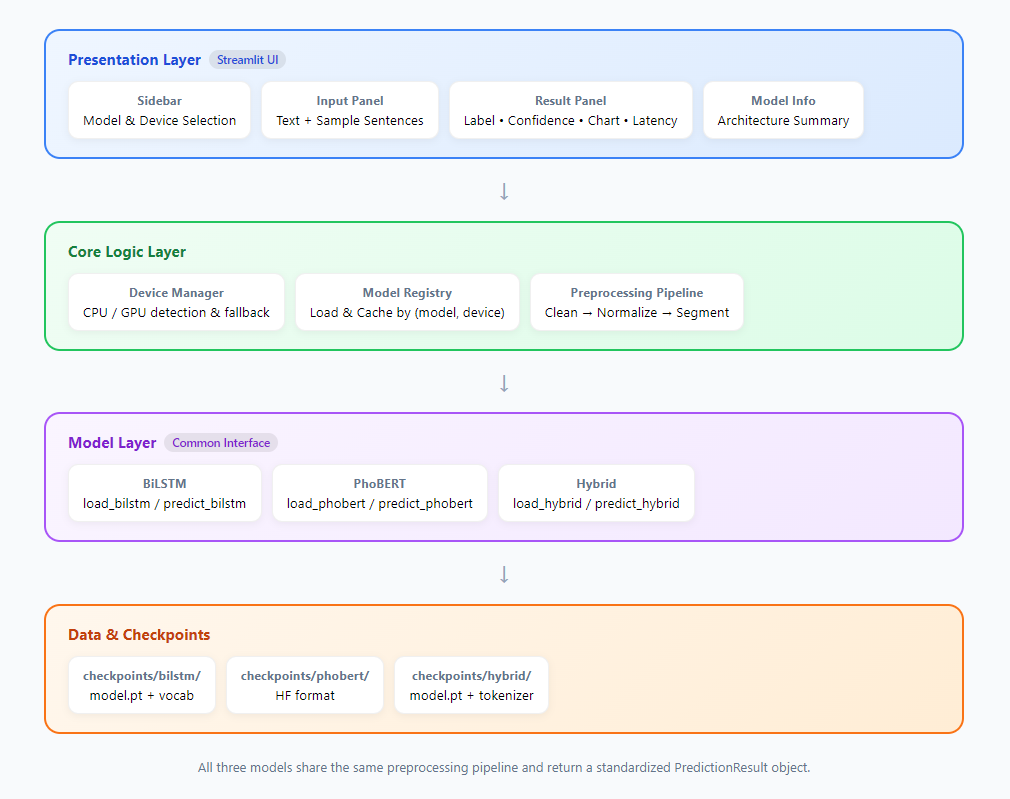
\includegraphics[width=0.95\textwidth]{figures/System_architecture.png}
    \caption{Overall architecture of the web-based sentiment analysis application. The system is organized into four layers: Presentation Layer (Streamlit UI), Core Logic Layer, Model Layer (with a common interface), and Data \& Checkpoints. All three models share the same preprocessing pipeline and return a standardized \texttt{PredictionResult} object.}
    \label{fig:app-architecture}
\end{figure}

\subsection{Backend Components}

Key backend components include:
\begin{itemize}
    \item \textbf{Device Manager} (\texttt{core/device\_manager.py}): Detects CUDA availability and resolves the computation device, with automatic fallback.
    \item \textbf{Preprocessing Pipeline} (\texttt{core/preprocessing\_pipeline.py}): Applies a consistent sequence of cleaning, normalization, and segmentation steps.
    \item \textbf{Model Registry} (\texttt{core/model\_registry.py}): Loads and caches models keyed by the pair (model name, device) to avoid redundant loading.
    \item \textbf{Model Modules} (\texttt{models/}): Separate implementations for BiLSTM, PhoBERT, and Hybrid PhoBERT-BiLSTM, each exposing \texttt{load\_*} and \texttt{predict\_*} functions that return a standardized \texttt{PredictionResult} object.
\end{itemize}

\subsection{Model Integration}

All three models implement a common interface defined in \texttt{models/base.py}:
\begin{itemize}
    \item \texttt{ModelBundle}: Encapsulates the loaded model and any auxiliary resources (vocabulary, tokenizer, configuration).
    \item \texttt{PredictionResult}: Contains the predicted label, confidence, probability dictionary, preprocessing latency, inference latency, and the processed text.
\end{itemize}

This design guarantees that the user interface remains completely agnostic to the internal differences among the three architectures.

\subsection{Data Flow}

The end-to-end data flow is as follows:
\begin{enumerate}
    \item User submits text and selects a model + device.
    \item The system validates the input and resolves the computation device.
    \item The selected model is loaded (or retrieved from cache).
    \item The input text passes through the shared preprocessing pipeline.
    \item The model performs inference and returns a \texttt{PredictionResult}.
    \item The result is rendered in the user interface together with latency metrics and model information.
\end{enumerate}

\subsection{Deployment Architecture}

The application is designed for local deployment. After cloning the repository and placing the trained checkpoints in the appropriate directories, the user simply runs:
\begin{verbatim}
streamlit run app.py
\end{verbatim}
The application then becomes available at \texttt{http://localhost:8501}. No external server or cloud service is required, making it suitable for offline demonstration and resource-constrained environments.

\section{Application Workflow}

The complete user workflow consists of the following sequential stages:

\begin{figure}[H]
    \centering
    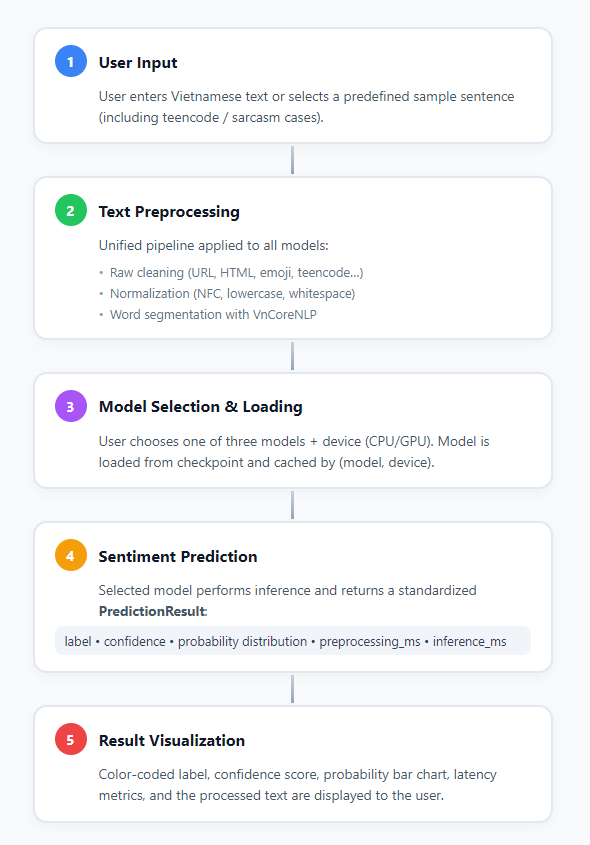
\includegraphics[width=0.85\textwidth]{figures/app_workflow.png}
    \caption{Application workflow of the web-based sentiment analysis system. The process consists of five sequential stages: (1) User Input, (2) Text Preprocessing, (3) Model Selection \& Loading, (4) Sentiment Prediction, and (5) Result Visualization.}
    \label{fig:app-workflow}
\end{figure}

\begin{enumerate}
    \item \textbf{User Input:} The user enters text or selects a sample sentence.
    \item \textbf{Text Preprocessing:}
          \begin{itemize}
              \item Stage 1 (optional raw cleaning for user-typed text): removal of URLs, HTML tags, emoji normalization, teencode replacement, etc.
              \item Stage 2 (mandatory, identical to training): Unicode normalization, lowercasing, and word segmentation using VnCoreNLP \cite{vu2018vncorenlp}.
          \end{itemize}
    \item \textbf{Model Selection \& Loading:} The chosen model is loaded onto the selected device (CPU or GPU) and cached.
    \item \textbf{Sentiment Prediction:} The preprocessed text is fed to the model, which returns the label, confidence, and probability distribution.
    \item \textbf{Result Visualization:} The interface displays the predicted sentiment with color coding, a probability bar chart, and separate preprocessing and inference latency values.
\end{enumerate}

A progress overlay informs the user of the current stage (input validation $\rightarrow$ model loading $\rightarrow$ preprocessing $\rightarrow$ inference).

\section{User Interface Design}

The interface is deliberately minimal and focused on clarity.

\begin{figure}[H]
    \centering
    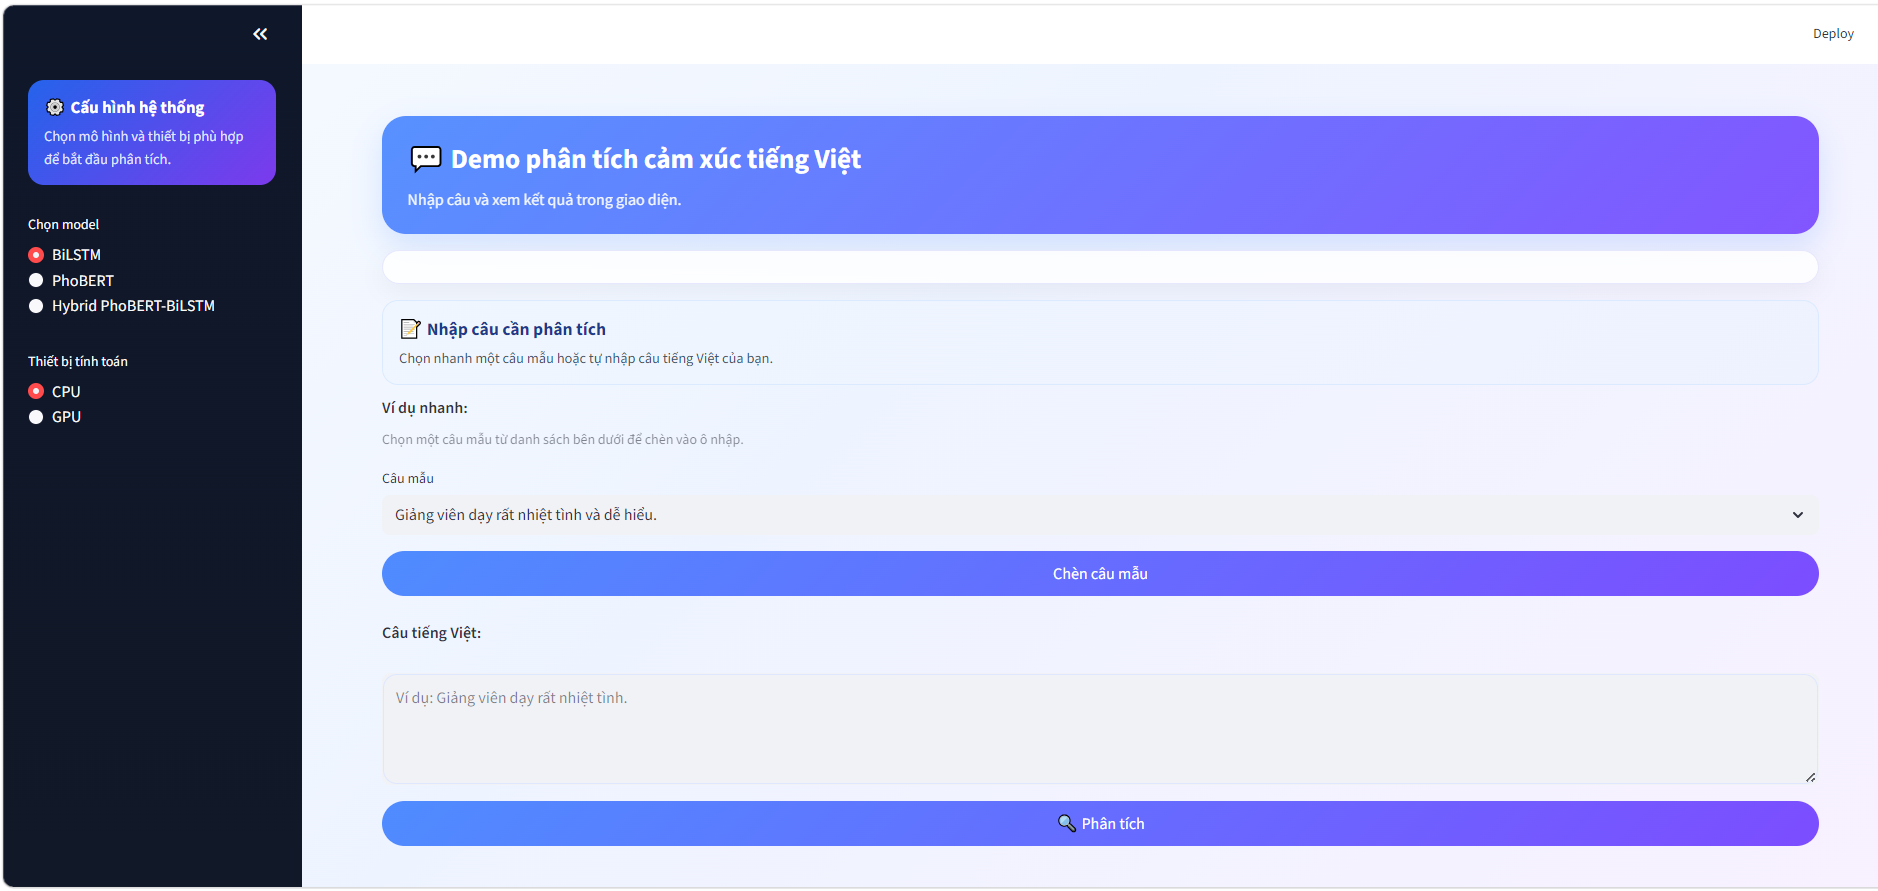
\includegraphics[width=0.95\textwidth]{figures/ui_home.png}
    \caption{Main user interface of the web-based sentiment analysis application. The left sidebar allows users to select the model (BiLSTM, PhoBERT, or Hybrid PhoBERT-BiLSTM) and the computation device (CPU/GPU). The main panel provides text input, sample sentence selection, and the analysis button.}
    \label{fig:ui-home}
\end{figure}

\begin{figure}[H]
    \centering
    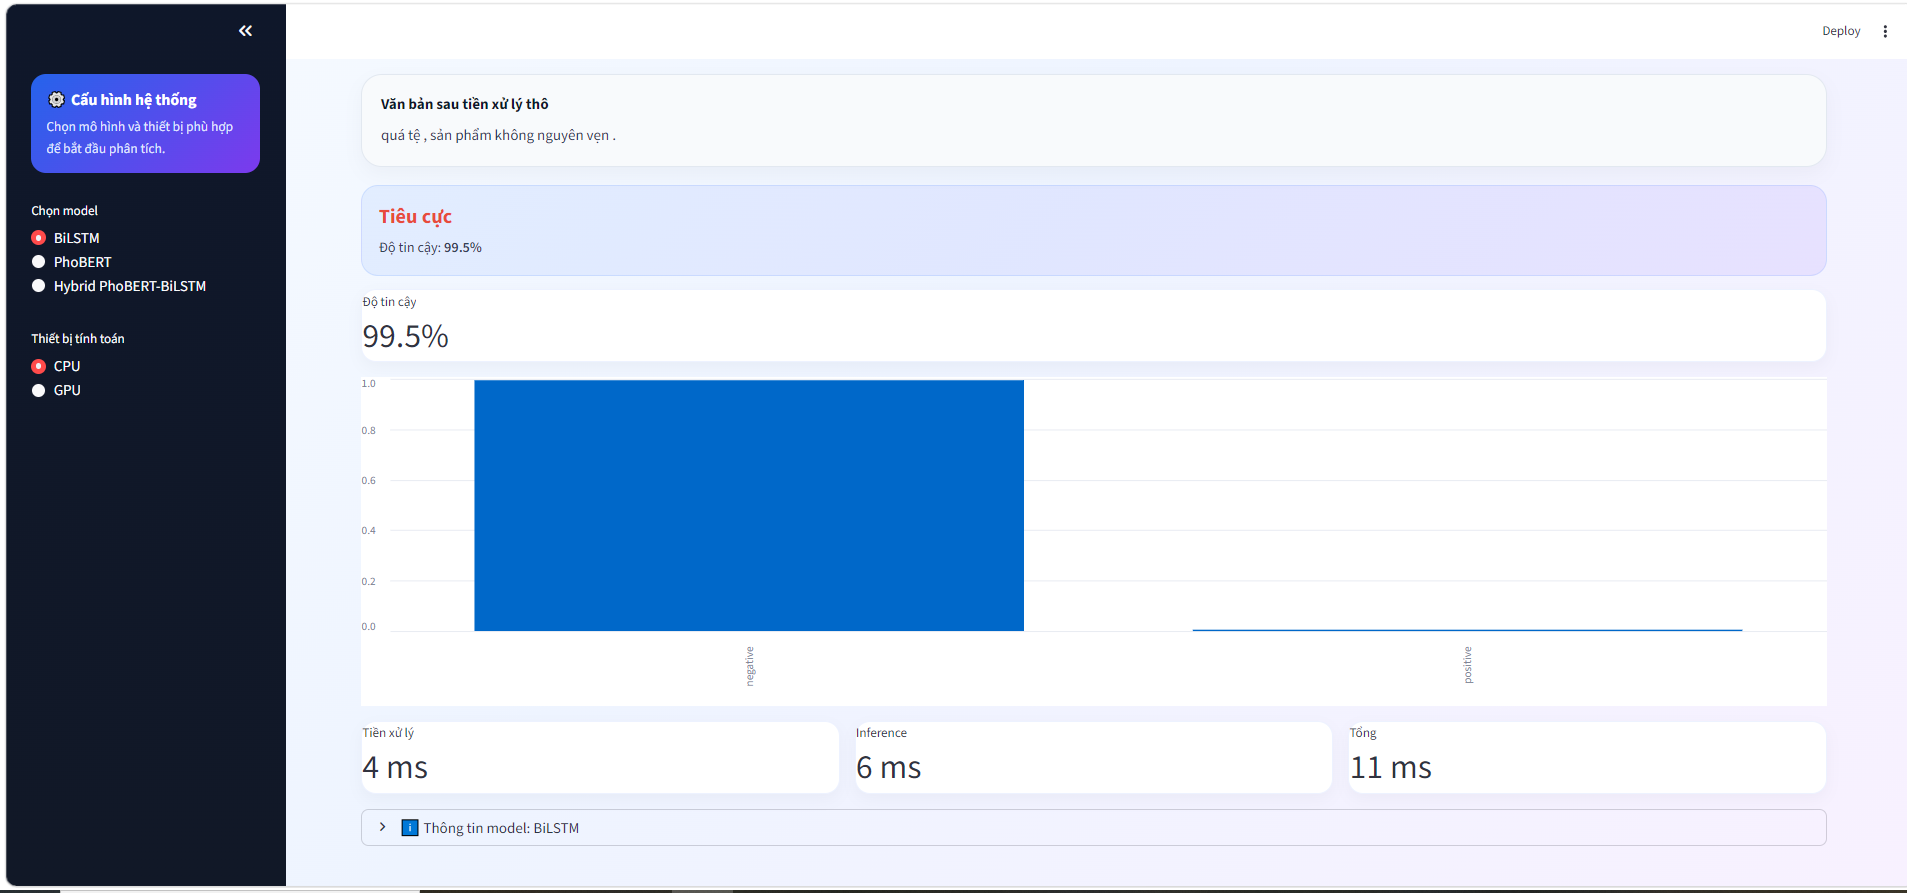
\includegraphics[width=0.95\textwidth]{figures/ui_prediction.png}
    \caption{Prediction result interface. After analysis, the system displays the preprocessed text, the predicted sentiment label with confidence score, a probability bar chart, and detailed latency metrics (preprocessing time, inference time, and total time). In this example, the BiLSTM model classifies the input as Negative with 99.5\% confidence.}
    \label{fig:ui-prediction}
\end{figure}

\begin{itemize}
    \item \textbf{Home / Hero Section:} A gradient banner introduces the purpose of the application.
    \item \textbf{Sidebar (Configuration):}
          \begin{itemize}
              \item Radio buttons for model selection (BiLSTM, PhoBERT, Hybrid PhoBERT-BiLSTM).
              \item Radio buttons for device selection (CPU / GPU) with informative captions when CUDA is unavailable.
          \end{itemize}
    \item \textbf{Input Panel:} A multi-line text area accompanied by quick-select sample sentences covering diverse linguistic phenomena.
    \item \textbf{Prediction Interface:} A prominent ``Analyze'' button triggers the full pipeline.
    \item \textbf{Result Presentation:}
          \begin{itemize}
              \item Color-coded predicted label (green for Positive, red for Negative).
              \item Confidence percentage.
              \item Probability bar chart.
              \item Three latency metrics (preprocessing, inference, total).
              \item Display of the text after preprocessing for transparency.
          \end{itemize}
    \item \textbf{Model Information Panel:} Brief architectural notes about the currently active model.
\end{itemize}

Custom CSS is applied to create a modern, clean visual appearance while remaining fully functional.

\section{System Implementation}

\subsection{Technology Stack}

\begin{table}[htbp]
    \centering
    \caption{Technology stack of the web-based application.}
    \label{tab:tech-stack}
    \begin{tabular}{ll}
        \hline
        \textbf{Component} & \textbf{Technology}                                               \\
        \hline
        Web framework      & Streamlit $\geq$ 1.36 \cite{streamlit2024}                        \\
        Deep learning      & PyTorch $\geq$ 2.2 \cite{paszke2019pytorch}                       \\
        Transformer models & Hugging Face Transformers $\geq$ 4.41 \cite{wolf2020transformers} \\
        Word segmentation  & py-vncorenlp + VnCoreNLP \cite{vu2018vncorenlp}                   \\
        Text utilities     & underthesea, emoji, pandas                                        \\
        Language           & Python $\geq$ 3.9                                                 \\
        \hline
    \end{tabular}
\end{table}

\subsection{Streamlit Implementation}

The application is structured as a single-page Streamlit app with modular UI components located in the \texttt{ui/} package. Session state is used only for device-selection feedback; model caching is handled independently by the model registry to avoid Streamlit’s re-execution side effects.

\subsection{Model Loading Strategy}

Models are loaded lazily and cached by the key \texttt{(model\_name, device)}. Changing either the model or the device triggers a fresh load, guaranteeing correctness while minimizing redundant computation. Checkpoint directories follow a fixed layout:
\begin{verbatim}
checkpoints/
├── bilstm/     (model.pt, vocab.json, config.json)
├── phobert/    (Hugging Face format + inference_config.json)
└── hybrid/     (model.pt, config.json, tokenizer/)
\end{verbatim}

\subsection{Runtime Optimization}

\begin{itemize}
    \item Model and tokenizer objects are kept in memory after the first load.
    \item Preprocessing and inference latencies are measured separately and reported to the user.
    \item A soft latency warning threshold is applied according to the selected device (higher tolerance on CPU).
\end{itemize}

\subsection{Project Structure}

\begin{verbatim}
VietSentimetApp/
├── app.py                      # Entry point
├── config/settings.py          # Model registry, labels, paths
├── core/
│   ├── text_cleaning.py
│   ├── normalization.py
│   ├── segmentation.py
│   ├── preprocessing_pipeline.py
│   ├── device_manager.py
│   └── model_registry.py
├── models/
│   ├── base.py
│   ├── bilstm_model.py
│   ├── phobert_model.py
│   └── hybrid_model.py
├── ui/
│   ├── sidebar.py
│   ├── input_panel.py
│   ├── result_panel.py
│   └── model_info_panel.py
├── checkpoints/                # (not committed)
├── requirements.txt
└── README.md
\end{verbatim}

\section{Case Study and Demonstration}

\subsection{Sample Prediction Cases}

The application includes five carefully chosen sample sentences that illustrate different linguistic challenges:
\begin{itemize}
    \item Standard positive feedback
    \item Standard negative feedback
    \item Neutral-sounding but weakly polarized text
    \item Sarcastic comment
    \item Teencode-heavy informal text
\end{itemize}

Users can also input arbitrary sentences, including those containing emojis, repeated characters, or mixed teencode.

\subsection{Comparison between the Three Models}

Because the same preprocessing pipeline and the same input text are used for every model, differences in predicted label or confidence can be attributed primarily to architectural characteristics. In typical interactive sessions, users observe that:
\begin{itemize}
    \item PhoBERT and the Hybrid model tend to produce higher confidence scores on well-formed academic-style feedback.
    \item BiLSTM is noticeably faster on CPU.
    \item On highly informal or sarcastic inputs, the three models may occasionally diverge, providing qualitative insight into their respective strengths and limitations.
\end{itemize}

\subsection{Practical Usage Scenarios}

Typical usage scenarios include:
\begin{itemize}
    \item Rapid inspection of model behavior on newly collected student feedback.
    \item Classroom demonstration of the effect of preprocessing and model choice.
    \item Preliminary testing of real-world social-media comments before larger-scale offline evaluation.
    \item Latency benchmarking on the target deployment hardware (CPU vs.\ GPU).
\end{itemize}

\section{Chapter Summary}

This chapter has presented a complete web-based demonstration application that integrates the three models developed and evaluated in this thesis. By providing a unified preprocessing pipeline, a consistent prediction interface, and transparent latency reporting, the application allows users to interactively explore the practical behavior of BiLSTM, PhoBERT, and Hybrid PhoBERT-BiLSTM on Vietnamese text. The modular design and local deployment model make the system suitable for both research exploration and educational demonstration, thereby complementing the quantitative experimental results reported in Chapter~4.

The next chapter discusses the broader implications of the experimental findings and the practical trade-offs observed when moving from offline evaluation to interactive deployment.


\chapter{Discussion}

\section{Discussion of Research Questions}

\subsection{Discussion of RQ1}
\textbf{RQ1:} To what extent does the Hybrid PhoBERT-BiLSTM architecture outperform standalone models (BiLSTM and PhoBERT) in classifying Vietnamese sentiment?

The experimental results presented in Chapter~4 provide a nuanced answer to RQ1. On the in-domain UIT-VSFC test set, the Hybrid PhoBERT-BiLSTM model does \textit{not} outperform standalone PhoBERT: it achieves a Macro-F1 of 97.58\%, 0.61 percentage points below PhoBERT's 98.19\% (Section~4.2). It does, however, clearly outperform standalone BiLSTM, by 2.41 percentage points. This pattern holds, and becomes more pronounced, under cross-domain evaluation (Section~4.3): Hybrid outperforms BiLSTM by 9.48 percentage points on AIVIVN-2019 (79.81\% vs.\ 70.33\% Macro-F1), while still trailing PhoBERT by 3.82 percentage points. Thus, RQ1 is answered asymmetrically: the Hybrid architecture consistently and substantially outperforms the from-scratch BiLSTM baseline, but does not surpass standalone, fully fine-tuned PhoBERT on raw accuracy in either evaluation setting. Its practical advantage instead lies in retaining most of PhoBERT's accuracy at a reduced computational cost (Section~4.5) --- a trade-off examined further under RQ3.

\subsection{Discussion of RQ2}
\textbf{RQ2:} How effective is the combination of PhoBERT's contextual embedding and BiLSTM's sequential memory in handling Vietnamese linguistic complexities (e.g., word ambiguity, negation)?

Because the Hybrid model uses a frozen, truncated (8-of-12-layer) PhoBERT encoder combined with a trainable BiLSTM (Section~3.4.3), the sequential layer must extract usable structure from a fixed, general-domain representation rather than from a representation co-adapted to the sentiment task, as in fully fine-tuned PhoBERT. The results suggest this combination is moderately, but not fully, effective. Cross-domain generalization results (Section~4.3) show that the Hybrid model's Macro-F1 degradation (17.77\% $\pm$ 3.44) is substantially smaller than BiLSTM's (24.83\% $\pm$ 2.29), indicating that PhoBERT's contextual embeddings do transfer useful semantic information to the BiLSTM layer even without joint fine-tuning. However, the Hybrid model's higher variance across seeds, relative to PhoBERT's (1.18), suggests that this combination is less stable than end-to-end fine-tuning at consistently resolving harder linguistic phenomena such as negation and word-sense ambiguity (Section~1.1). The sequence-length analysis (Section~4.4) reinforces this: the Hybrid model's performance on Short, context-poor sentences is consistently weaker than PhoBERT's across all three test sets, implying that when little surrounding context is available to compensate for the frozen encoder's fixed representations, the BiLSTM layer alone cannot fully resolve ambiguity that end-to-end fine-tuning would otherwise learn to handle.

\subsection{Discussion of RQ3}
\textbf{RQ3:} What is the trade-off between classification accuracy and computational latency when deploying these models in a real-world application context?

Section~4.5 quantifies this trade-off directly. BiLSTM offers by far the lowest latency (6.15 ms CPU, 1.09 ms GPU) but the weakest accuracy and generalization of the three models. PhoBERT offers the highest accuracy across every evaluation setting but at substantially higher latency (2227.64 ms CPU, 22.35 ms GPU) --- roughly 360$\times$ and 20$\times$ slower than BiLSTM, respectively. The Hybrid architecture is positioned as an explicit answer to this trade-off: relative to full PhoBERT, it reduces CPU latency by approximately 29\% and GPU latency by approximately 20\%, while sacrificing only 0.61 percentage points of in-domain Macro-F1 and retaining a meaningful share of cross-domain robustness (Section~4.3). For deployment contexts with strict latency constraints (Section~1.1: real-time banking or e-commerce sentiment monitoring), this makes the Hybrid model a more practical choice than full PhoBERT when BiLSTM's accuracy loss is unacceptable, though it does not eliminate the latency gap with BiLSTM by an order of magnitude. The choice among the three architectures therefore depends on where a given deployment scenario sits along this accuracy-latency spectrum, rather than any one model being uniformly optimal.

\section{Comparative Analysis of the Three Models}

While Section~6.1 addressed the three research questions directly, this section synthesizes the results of Chapters~3--4 into a broader comparative profile of each architecture, highlighting where each model's design choices translate into a genuine practical advantage.

\subsection{Strengths of BiLSTM}
BiLSTM's principal strength is \textbf{computational efficiency}: at approximately 2.1 million parameters (Section~3.4.1) and 6.15 ms CPU / 1.09 ms GPU inference latency (Section~4.5), it is by a wide margin the cheapest of the three models to train and deploy, requiring no pretrained checkpoint and no GPU for practical inference. Despite relying entirely on randomly initialized embeddings, it achieves a respectable 95.17\% Macro-F1 in-domain (Section~4.2), and on UIT-VSFC's predominantly short, single-topic sentences (Section~3.2.1), its performance gap relative to the pretrained-representation models remains comparatively small (2.4--3.0 percentage points). BiLSTM is therefore best suited to resource-constrained deployment contexts operating within, or close to, the training domain, where its low cost outweighs its weaker generalization capability.

\subsection{Strengths of PhoBERT}
PhoBERT's principal strength is \textbf{accuracy and generalization}: it achieves the highest Macro-F1 in every evaluation setting examined in this study --- in-domain (98.19\%), cross-domain on AIVIVN-2019 (83.63\%), and real-world on the YouTube wild test set (87.91\%) --- and does so with the lowest cross-seed variance among the three models (Sections~4.2--4.3, 4.6). Its full end-to-end fine-tuning on UIT-VSFC allows all 12 Transformer layers to adapt jointly to the sentiment task, and its pretraining on 20GB of general-domain Vietnamese text \cite{nguyen2020phobert} evidently transfers well beyond the academic-feedback domain it was fine-tuned on, as shown by its comparatively small performance degradation out-of-domain (Section~4.3). This makes PhoBERT the model of choice whenever accuracy and robustness to distribution shift outweigh latency and computational cost.

\subsection{Strengths of Hybrid PhoBERT-BiLSTM}
Hybrid PhoBERT-BiLSTM's principal strength is \textbf{balancing accuracy against computational cost}. By freezing and truncating the PhoBERT encoder to its first 8 of 12 layers (Section~3.4.3), it reduces inference latency relative to full PhoBERT by approximately 29\% (CPU) and 20\% (GPU), while sacrificing only 0.61 percentage points of in-domain Macro-F1 and retaining a meaningful share of PhoBERT's cross-domain robustness (Section~4.3, 4.5). Unlike BiLSTM, it still benefits from pretrained contextual representations, and unlike PhoBERT, it requires no gradient updates to the (large majority of the) Transformer encoder during training, reducing training-time computational demand as well. Its strength is therefore not outright superiority on any single metric, but rather occupying a favorable middle position on the accuracy-latency spectrum established under RQ3 (Section~6.1).

\subsection{Performance versus Computational Cost}
Table~\ref{tab:tradeoff-summary} consolidates the core accuracy-cost trade-off across all three models, combining in-domain Macro-F1 (Table~\ref{tab:uitvsfc-results}) with CPU/GPU latency (Table~\ref{tab:latency}).

\begin{table}[htbp]
    \centering
    \caption{Summary of accuracy-latency trade-off across the three models.}
    \label{tab:tradeoff-summary}
    \begin{tabular}{lccc}
        \hline
        \textbf{Model}        & \textbf{In-domain F1 (\%)} & \textbf{CPU Latency (ms)} & \textbf{GPU Latency (ms)} \\
        \hline
        BiLSTM                & 95.17                      & 6.15                      & 1.09                      \\
        Hybrid PhoBERT-BiLSTM & 97.58                      & 1573.21                   & 17.82                     \\
        PhoBERT               & 98.19                      & 2227.64                   & 22.35                     \\
        \hline
    \end{tabular}
\end{table}

No single model dominates all three axes simultaneously: improving accuracy consistently costs latency, and vice versa. This confirms that architecture selection in Vietnamese sentiment analysis --- and, by extension, in similarly resource-constrained NLP settings --- should be driven by the specific latency and accuracy requirements of the target deployment context (Section~1.1), rather than by in-domain benchmark accuracy alone, a concern largely absent from prior Vietnamese sentiment analysis literature (Research Gap 4, Section~2.2).

\section{Practical Implications}

The results presented in Chapters~4--5 have direct relevance to the practical motivations for this study outlined in Section~1.1: the growing need for automated Vietnamese sentiment analysis across e-commerce, banking, and education sectors.

\subsection{Applications in E-commerce}
With Vietnam's e-commerce sector sustaining growth of over 25\% annually and a market scale of \$25 billion \cite{vecom_2024}, the volume of user-generated reviews and comments increasingly exceeds what manual moderation can process (Section~1.1). The cross-domain evaluation on AIVIVN-2019 (Section~4.3), itself a corpus of e-commerce product reviews, is directly relevant here: PhoBERT's 83.63\% Macro-F1 and comparatively small degradation from in-domain performance suggest it is well suited to classifying real e-commerce feedback without requiring retraining on platform-specific data, while the Hybrid model offers a reduced-latency alternative for higher-throughput moderation pipelines.

\subsection{Applications in Banking}
Vietnamese banks are increasingly deploying social listening to monitor brand health and detect customer complaints in near real time \cite{reputa_2024}. In this context, inference latency is often as critical as accuracy, since customer complaints frequently require timely escalation. The latency figures established in Section~4.5 --- BiLSTM at 1.09 ms and Hybrid PhoBERT-BiLSTM at 17.82 ms on GPU --- both fall well within real-time processing requirements, making either a more suitable choice than full PhoBERT (22.35 ms) for high-volume, latency-sensitive banking applications, with the accuracy trade-off between them depending on the acceptable error tolerance for a given monitoring task.

\subsection{Applications in Education}
As the source domain of the UIT-VSFC corpus itself, educational institutions represent the most directly validated application context in this study (Section~4.2). Automated analysis of student feedback for accreditation and quality-improvement purposes \cite{younet_2023} can rely on any of the three models with confidence, given their consistently high in-domain performance (95.17--98.19\% Macro-F1); PhoBERT is the natural choice where maximal accuracy is prioritized, while BiLSTM's minimal computational footprint suits institutions with limited infrastructure.

\subsection{Applications in Social Listening}
Beyond banking specifically, general-purpose social listening --- monitoring public sentiment across social media platforms for brand or reputation management \cite{younet_2023} --- most closely resembles the conditions of the YouTube wild test set evaluated in Section~4.6: informal, unmoderated, real-world text. PhoBERT's strong performance in this setting (87.91\% Macro-F1) indicates that pretrained contextual representations are particularly valuable when processing genuinely uncontrolled social media language, reinforcing the general finding (Section~6.1, RQ2) that fine-tuned contextual embeddings generalize across register, not only topical domain.

\subsection{Recommendations for Real-world Deployment}
Synthesizing the above, this study offers the following practical deployment guidance:
\begin{itemize}
    \item \textbf{Prioritize PhoBERT} when classification accuracy and robustness to unfamiliar domains or registers are the primary requirement, and GPU inference infrastructure is available (e.g., offline batch analysis of banking or e-commerce reviews).
    \item \textbf{Prioritize BiLSTM} when computational resources are severely constrained (e.g., edge deployment, CPU-only environments) and the input distribution remains reasonably close to the training domain.
    \item \textbf{Prioritize Hybrid PhoBERT-BiLSTM} when a deployment context requires a balance between the two --- meaningfully better accuracy and generalization than BiLSTM, at a meaningfully lower computational cost than full PhoBERT --- such as real-time social listening or moderate-throughput customer feedback pipelines (Section~6.2).
\end{itemize}

\section{Limitations of the Study}

While this study provides a controlled, multi-dimensional comparison of three Vietnamese sentiment analysis architectures, several limitations should be acknowledged when interpreting its findings.

\subsection{Dataset Limitations}
The primary training resource, UIT-VSFC, consists of academic course-feedback sentences collected over three academic years at a single Vietnamese university (Section~3.2.1), and is predominantly composed of short sentences (over 83\% under 15 words, Section~3.2.1). All three models are therefore trained exclusively on this relatively narrow linguistic distribution, and their in-domain performance (Section~4.2) reflects proficiency on this specific style of text rather than Vietnamese sentiment expression in general. Additionally, the AIVIVN-2019 cross-domain test set is evaluated via a fixed-size random subsample per seed (Section~3.2.2, Section~3.8) rather than its full 3,217-review extent, and the YouTube wild test set is limited to comments from a single video (Section~3.2.3), whose specific topic (a patriotic tribute video) plausibly shaped both its class distribution (62.5\% Positive) and its linguistic characteristics in ways that may not generalize to YouTube comments on other topics.

\subsection{Binary Sentiment Classification}
Following the scope established in Section~1.3.1, this study excludes the Neutral class present in the original UIT-VSFC corpus, framing sentiment classification as a binary Positive/Negative task. While this decision was motivated by the Neutral class's small proportion (4.01\% of the training set, Section~3.2.1) and its comparatively poor baseline classifiability in prior work \cite{nguyen2018uitvsfc}, it necessarily limits the applicability of this study's findings to real-world scenarios where Neutral or mixed-sentiment content is common and cannot simply be discarded --- for instance, purely factual customer service inquiries or ambiguous social media comments that express no clear polarity.

\subsection{Limited Evaluation Domains}
Although this study evaluates cross-domain generalization across three distinct sources (UIT-VSFC, AIVIVN-2019, and YouTube comments), all three remain within a broadly similar register of consumer- or citizen-generated Vietnamese text. Domains explicitly motivated in Section~1.1 --- such as banking customer service transcripts or e-learning platform feedback --- are not directly evaluated, and the practical implications discussed in Section~6.3 for these domains are therefore extrapolated from related, but not identical, evaluation settings rather than directly measured.

\subsection{Computational Constraints}
All experiments in this study were conducted on Google Colab's free tier, using a single NVIDIA Tesla T4 GPU (Section~3.6). This constrained the choice of the maximum number of training epochs (particularly for PhoBERT, capped at 5, Table~\ref{tab:training-hyperparams}) and precluded experimentation with larger PhoBERT variants (e.g., \texttt{phobert-large}) or more extensive hyperparameter search, any of which might further improve the reported results. Additionally, GPU memory consumption and total training time were not systematically measured (Section~4.5), limiting the completeness of the computational cost analysis relative to the inference-latency and parameter-count dimensions that were measured.

\section{Future Work}

The limitations identified in Section~6.4, together with observations from the experimental results in Chapter~4, motivate several concrete directions for future research, each addressing a specific, evidence-grounded gap in the present study rather than a generic extension.

\subsection{Qualitative Error Analysis}
While this study's evaluation is thorough at the aggregate level --- spanning overall Accuracy/Macro-F1, per-domain generalization, and sequence-length breakdowns (Sections~4.2--4.4) --- it does not include example-level inspection of individual misclassifications. A systematic error analysis, categorizing misclassified samples by linguistic phenomenon (negation, sarcasm, slang and teencode, long or syntactically complex sentences, and domain-specific vocabulary), would help determine \textit{why} the observed performance gaps between BiLSTM, PhoBERT, and Hybrid PhoBERT-BiLSTM occur (Section~6.1, RQ2), rather than only quantifying \textit{that} they occur. Such analysis is particularly warranted given this study's finding that Short, context-poor sentences are disproportionately difficult for the Hybrid model out-of-domain (Section~4.4): example-level inspection could clarify whether this stems specifically from unresolved negation, insufficient context for disambiguation, or another mechanism.

\subsection{Multi-class Sentiment Classification}
This study's binary scope (Section~1.3.1) was adopted primarily due to the Neutral class's small representation and comparatively low classifiability in UIT-VSFC (Section~6.4). Future work should revisit the original three-class formulation (Positive/Negative/Neutral), ideally combined with class-imbalance mitigation techniques (e.g., class-weighted loss or resampling), to establish whether the architectural rankings observed in this study --- particularly PhoBERT's and Hybrid's generalization advantage over BiLSTM (Section~4.3) --- persist when the additional difficulty of distinguishing Neutral from weak Positive or Negative sentiment is reintroduced.

\subsection{Aspect-based Sentiment Analysis}
The sentence-level classification task examined in this study does not distinguish sentiment expressed toward different aspects within the same text (e.g., a review praising delivery speed while criticizing product quality). Given that UIT-VSFC additionally provides topic-based annotations (Lecturer, Curriculum, Facility, Others) alongside its sentiment labels \cite{nguyen2018uitvsfc}, a natural extension is to jointly model aspect and sentiment, enabling finer-grained analysis directly relevant to the practical applications discussed in Section~6.3 (e.g., disentangling specific complaint categories in e-commerce or banking feedback, rather than a single overall polarity).

\subsection{Larger Vietnamese Language Models}
This study's Transformer-based models are restricted to \texttt{phobert-base} (Section~3.4.2--3.4.3), due to the computational constraints of the Google Colab free tier (Section~6.4). Future work should evaluate whether the accuracy and generalization advantages observed for PhoBERT over BiLSTM (Sections~4.2--4.3) scale further with larger pretrained Vietnamese encoders (e.g., \texttt{phobert-large}), and whether the Hybrid architecture's layer-truncation strategy (Section~3.4.3) remains an effective cost-reduction technique when applied to a larger base encoder, or whether the accuracy-latency trade-off characterized in Section~6.2 shifts substantially at greater model scale.

\subsection{LLM-based Sentiment Analysis}
This study already incorporates large language models indirectly, as annotators in the YouTube wild test set labeling procedure (Section~3.2.3). A direct extension is to evaluate general-purpose LLMs (used via prompting, rather than as annotators) as sentiment classifiers themselves, under the same evaluation protocol established in this study (Sections~3.7--3.8), to determine whether prompt-based LLM classification can match or exceed the fine-tuned, task-specific models evaluated here --- particularly on the out-of-domain and real-world test sets (Sections~4.3, 4.6) where such models' broad pretraining may offer a generalization advantage analogous to, but potentially exceeding, that observed for PhoBERT.

\subsection{More Diverse Real-world Datasets}
As discussed in Section~6.4, this study's real-world evaluation is limited to comments from a single YouTube video, and its cross-domain evaluation to a single e-commerce review dataset. Future work should extend the domain-generalization evaluation strategy established in Section~3.8 to a broader and more diverse set of real-world sources --- multiple YouTube videos spanning different topics and audiences, other social media platforms, and additional application domains explicitly motivated in Section~1.1 (banking, education) but not directly evaluated in this study --- to establish whether the generalization rankings observed here (Section~4.3, 4.6) hold consistently across a wider range of real-world Vietnamese text.

\chapter{Conclusion}

\section{Research Summary}

\subsection{Summary of Research Objectives}
This thesis set out to conduct a controlled, empirical comparison of three deep learning architectures --- BiLSTM, PhoBERT, and a proposed Hybrid PhoBERT-BiLSTM model --- for Vietnamese Sentiment Analysis, guided by three research questions concerning relative performance, the effectiveness of combining pretrained contextual embeddings with sequential modeling, and the trade-off between accuracy and computational cost (Section~1.2). This work was further motivated by four specific gaps identified in prior Vietnamese sentiment analysis literature: the absence of a unified comparison pipeline, limited analysis of sequence-length sensitivity, insufficient assessment of cross-domain generalization, and the general neglect of deployment-related efficiency metrics (Section~2.2).

\subsection{Summary of Methodology}
To address these objectives, this study trained and evaluated all three models under an identical, controlled pipeline (Chapter~3): a shared preprocessing procedure applied uniformly across datasets and architectures (Section~3.3), binary sentiment classification on the UIT-VSFC corpus (Section~3.2.1), repeated training across five random seeds for statistical reliability (Section~3.5), and evaluation spanning both predictive performance and computational efficiency (Section~3.7), across three test sets of increasing distributional distance from the training domain (Section~3.8).

\subsection{Summary of Experimental Findings}
The resulting experiments (Chapter~4) showed that PhoBERT achieves the strongest performance in every evaluation setting, followed by Hybrid PhoBERT-BiLSTM, with BiLSTM trailing both --- a gap that widens substantially under cross-domain and real-world evaluation relative to in-domain performance. Sequence-length analysis further revealed that this generalization advantage is not uniform across sentence lengths, and computational analysis confirmed a clear accuracy-latency trade-off, with the Hybrid architecture occupying a favorable middle position between the lightweight BiLSTM baseline and the more accurate but costlier PhoBERT baseline. A full discussion and interpretation of these findings is provided in Chapter~6.

\section{Main Contributions}

\subsection{Academic Contributions}
This thesis contributes to the Vietnamese sentiment analysis literature by directly addressing the four research gaps identified in Section~2.2. It presents, to the best of the author's knowledge, the first controlled, identical-pipeline comparison of BiLSTM, PhoBERT, and a Hybrid PhoBERT-BiLSTM architecture on a shared Vietnamese benchmark (Chapter~3--4); it introduces a sequence-length-based performance breakdown that reveals generalization behavior obscured by aggregate accuracy metrics alone (Section~4.4); it extends evaluation beyond the training domain to two independent out-of-domain test sets, quantifying --- rather than merely acknowledging --- the domain generalization gap for each architecture (Sections~4.3, 4.6); and it reports training time, inference latency, and parameter counts alongside predictive accuracy, providing a deployment-oriented efficiency analysis largely absent from prior work in this area (Section~4.5).

\subsection{Technical Contributions}
On the technical side, this thesis proposes and implements a Hybrid PhoBERT-BiLSTM architecture that departs from prior hybrid approaches by combining a \textit{frozen, layer-truncated} PhoBERT encoder (retaining 8 of 12 Transformer layers) with a trainable bidirectional LSTM operating over the full sequence of hidden states, rather than a single pooled representation (Section~3.4.3). This design is shown to recover most of full PhoBERT's in-domain and cross-domain performance while measurably reducing inference latency (Sections~4.2--4.3, 4.5), offering a concrete, empirically validated alternative to full end-to-end fine-tuning for resource-constrained deployment. This thesis additionally contributes a complete, LLM-assisted and human-verified labeling procedure for constructing labeled real-world social media test data without full manual dual-annotation (Section~3.2.3), and a working, deployable web-based application built on the best-performing configuration (Chapter~5).

\subsection{Practical Contributions}
Beyond its academic and technical findings, this thesis provides concrete, evidence-based deployment guidance for practitioners applying Vietnamese sentiment analysis in e-commerce, banking, education, and social listening contexts (Section~6.3), directly grounded in the accuracy-latency trade-offs quantified in this study rather than general architectural intuition. The resulting web-based application (Chapter~5) further demonstrates that the study's findings translate into a functioning, usable tool rather than remaining purely experimental.

\section{Conclusions}

\subsection{Answers to the Research Questions}
In brief --- with full discussion provided in Section~6.1 --- this study found that the Hybrid PhoBERT-BiLSTM architecture outperforms BiLSTM substantially, both in-domain and cross-domain, but does not surpass standalone, fully fine-tuned PhoBERT on raw accuracy (RQ1). The combination of PhoBERT's contextual embeddings with BiLSTM's sequential modeling proved moderately effective at transferring semantic representations without joint fine-tuning, though comparatively less stable than end-to-end fine-tuning on harder, context-poor inputs (RQ2). Finally, a clear and quantifiable trade-off exists between accuracy and computational latency across all three models, with the Hybrid architecture offering a deliberate, measurable compromise between the two (RQ3).

\subsection{Final Comparison of the Three Models}
Across all evaluation dimensions examined in this study --- in-domain accuracy, cross-domain and real-world generalization, sequence-length sensitivity, and computational efficiency (Chapter~4) --- no single model dominates uniformly. PhoBERT is the most accurate and most robust to distribution shift; BiLSTM is the most computationally efficient; and Hybrid PhoBERT-BiLSTM occupies a deliberate middle ground, trading a small amount of PhoBERT's accuracy for a meaningful reduction in inference cost (Section~6.2). The appropriate choice among the three therefore depends on the specific accuracy, latency, and resource constraints of the deployment context in question (Section~6.3), rather than any single architecture being universally optimal.

\subsection{Overall Conclusions}
This thesis has demonstrated that pretrained contextual representations are the primary driver of both accuracy and generalization in Vietnamese sentiment analysis, and that a substantial share of this benefit can be retained at reduced computational cost through architectural modifications such as encoder truncation and freezing, as implemented in the proposed Hybrid model. By evaluating all three architectures under an identical, controlled, and generalization-aware methodology, this study provides not only a performance ranking but an evidence-based framework for architecture selection under real-world constraints --- directly fulfilling the objective set out in Section~1.2 of producing a comprehensive, practical guide rather than a single best-performing model.

\section{Future Directions}

\subsection{Suggested Research Directions}
The research directions outlined in Section~6.5 --- multi-class classification, aspect-based sentiment analysis, larger Vietnamese language models, LLM-based sentiment analysis, and more diverse real-world datasets --- are not purely speculative extensions; each connects to an active, ongoing line of work in the Vietnamese NLP community. On aspect-based sentiment analysis specifically, recent work such as Vi-AbSQA \cite{viabsqa2024} has begun tackling fine-grained aspect-sentiment quadruple extraction for Vietnamese, suggesting that the topic-annotated structure already present in UIT-VSFC (Section~2.2) could be leveraged in a similar direction using the same corpus this thesis has built upon. On larger Vietnamese language models, the rapid emergence of PhoGPT \cite{nguyen2023phogpt}, VinaLLaMA \cite{nguyen2023vinallama}, and Vistral \cite{nguyen2023vistral} since 2023 demonstrates that substantially larger, Vietnamese-native pretrained models are now openly available and could be evaluated as drop-in replacements for \texttt{phobert-base} within this thesis's Hybrid architecture (Section~3.4.3), potentially clarifying whether the accuracy-efficiency trade-off characterized in Section~6.2 holds at greater model scale. On LLM-based sentiment analysis, a growing body of work evaluates general-purpose LLMs as zero- or few-shot sentiment classifiers via prompting rather than fine-tuning; this thesis's own use of LLMs as annotators (Section~3.2.3) is a preliminary, informal instance of this broader direction, and a systematic evaluation of this approach against the fine-tuned models compared in this thesis would be a natural and directly comparable extension.

\subsection{Potential Improvements}
Beyond entirely new research directions, several concrete refinements to this thesis's own methodology could be pursued without fundamentally changing its scope. The Hybrid architecture's layer-truncation strategy (Section~3.4.3) was fixed at 8 of 12 layers in this study; a systematic ablation across different truncation depths would clarify whether this specific configuration is close to optimal, or whether a different trade-off point along the accuracy-latency spectrum (Section~6.2) would better serve specific deployment contexts. Similarly, the fixed Short/Medium/Long sequence-length thresholds derived from UIT-VSFC's training distribution (Section~3.3.2) could be revisited using a domain-agnostic or adaptive thresholding scheme, potentially yielding a more balanced comparison when applied to out-of-domain data with substantially different length distributions (Section~4.4). Finally, given the computational constraints acknowledged in Section~6.4, repeating this study's experiments on non-free-tier compute would allow longer PhoBERT fine-tuning schedules and a systematic measurement of GPU memory consumption and total training time, completing the computational efficiency analysis begun in Section~4.5.

\subsection{Future Application Prospects}
The practical deployment guidance established in Section~6.3, together with the working web-based application presented in Chapter~5, points toward several concrete application prospects. As Vietnamese-native large language models such as PhoGPT and VinaLLaMA mature and become more efficient to serve \cite{nguyen2023phogpt, nguyen2023vinallama}, they may offer a future alternative to the PhoBERT-based architectures evaluated in this thesis for applications where the highest possible accuracy is required and infrastructure constraints are less restrictive (e.g., centralized social listening platforms for banking and e-commerce, Section~6.3). Conversely, for edge or mobile deployment where the BiLSTM and Hybrid models' lower computational footprint (Section~4.5) remains advantageous, continued refinement of efficient hybrid architectures --- combining compact recurrent components with increasingly capable but resource-constrained pretrained encoders --- represents a promising direction for making high-quality Vietnamese sentiment analysis accessible outside well-resourced cloud environments.




% References
\selectlanguage{english}
\cleardoublepage
\addcontentsline{toc}{chapter}{References}
\bibliographystyle{plain}
\bibliography{references}

% Appendices
\cleardoublepage
\appendix
\pagenumbering{arabic}
\setcounter{page}{1}
\end{document}